\chapter{Simulation Outcomes}\label{chap:simulationoutcomes}
In the following the load balancing algorithms are abbreviated. The Single-Proposal Deal-Agreement-Based algorithm is abbreviated as DAB, the Push-Pull Sum algorithm is abbreviated as PPS and the Adaptive Threshold Push-Pull-Sum algorithm is abbreviated as ATPPS. The simulation outcomes are presented in plots, mostly log-log or log-linear graphs (logs for the mean squared error are base 10), since the mean squared error values vary a lot over the 100 rounds of simulation. Figures \ref{fig:completegrapslopes}, <slopes images referencing>  depict the slopes for three distinct regions (of the x-axis) and the general slope over all the 100 rounds. For each algorithm the function that distributes the mean squared error over the rounds is model fitted with the models of linear regression, polynomial regression, exponential decay or logarithmic regression, depending on the best-fit.

\textbf{Linear Regression}: The linear regression fits $MSE_r=m*r+b$ to the data. Where $m$ is the slope: $\frac{\Delta MSE}{\Delta r}$. In the case of load balancing the slope is mostly negative, meaning that for each round, the $MSE_r$ decreases in comparison to the $MSE_r-1$, the mean squared error of the previous round. $b$ is the mean squared error, in round 0, so in that round where the network is initialized in our experiments. In round 0 the mean squared error is calculated with the unbalanced network, so $MSE_0$ is the initial mean squared error, where no load balancing is applied yet. The 

\textbf{Polynomial Regression}: The polynomial model $MSE_r=a_0+a_1*r+a_2*r^{2}+a_3*r^{3}+...+a_n*r^{n}$ is a model where the mean squared error reduction per round follows a power law relationship. It captures non-linear relationships between the independent variable $r$ and dependent variable $MSE_r$ \cite{MotulskyDataFitting}. Polynomial regression can model non-linear trends like diminishing returns (e.g., rapid MSE reduction initially, then slower reduction). It fits the curvature of MSE decay, even if it's not strictly exponential or linear. Higher-degree polynomials can capture intricate patterns in the reduction of MSE over rounds.

\textbf{Exponential Regression}: The exponential regression model fits $MSE_r=a*e^{-br}$ to the data. Exponential models capture the initially steep drop in mean squared error at early rounds, followed by slower reductions in later rounds. The exponential decay model is also an non-linear model. The initial value of the mean squared error is captured by $a$. In the initializing round where $r=0$, $MSE_r=a*e^{b*0}$ evaluates to $MSE_r=a$. Larger $a$ values indicate larger initial error in the network. The decay rate is captured by $b$. The $b$ value determines how quickly the MSE decreases per round $r$. For the exponential decay model $b$ is negative. A larger negative value for $b$ indicates a faster error reduction in the network, while values closer to 0 indicate slower error reduction.

\textbf{Logarithmic Regression}: The logarithmic regression models data as $MSE_r=a+b*\log{(r)}$. $a$ is the initial mean squared error, when $\log{(r)}=0$. $b$ is the rate of reduction per unit of logarithmic increase in rounds. A large positive $b$ decreases the error faster.

\section{Complete Graph}\label{sec:completeGraph}
Figures \ref{fig:completegraphMSEperRoundLogLog} show the mean squared error reduction over the rounds for the three load balancing algorithms simulated on the complete graph on a log-log graph.

%\begin{figure}[h]
%    \centering
%    \scalebox{0.5}{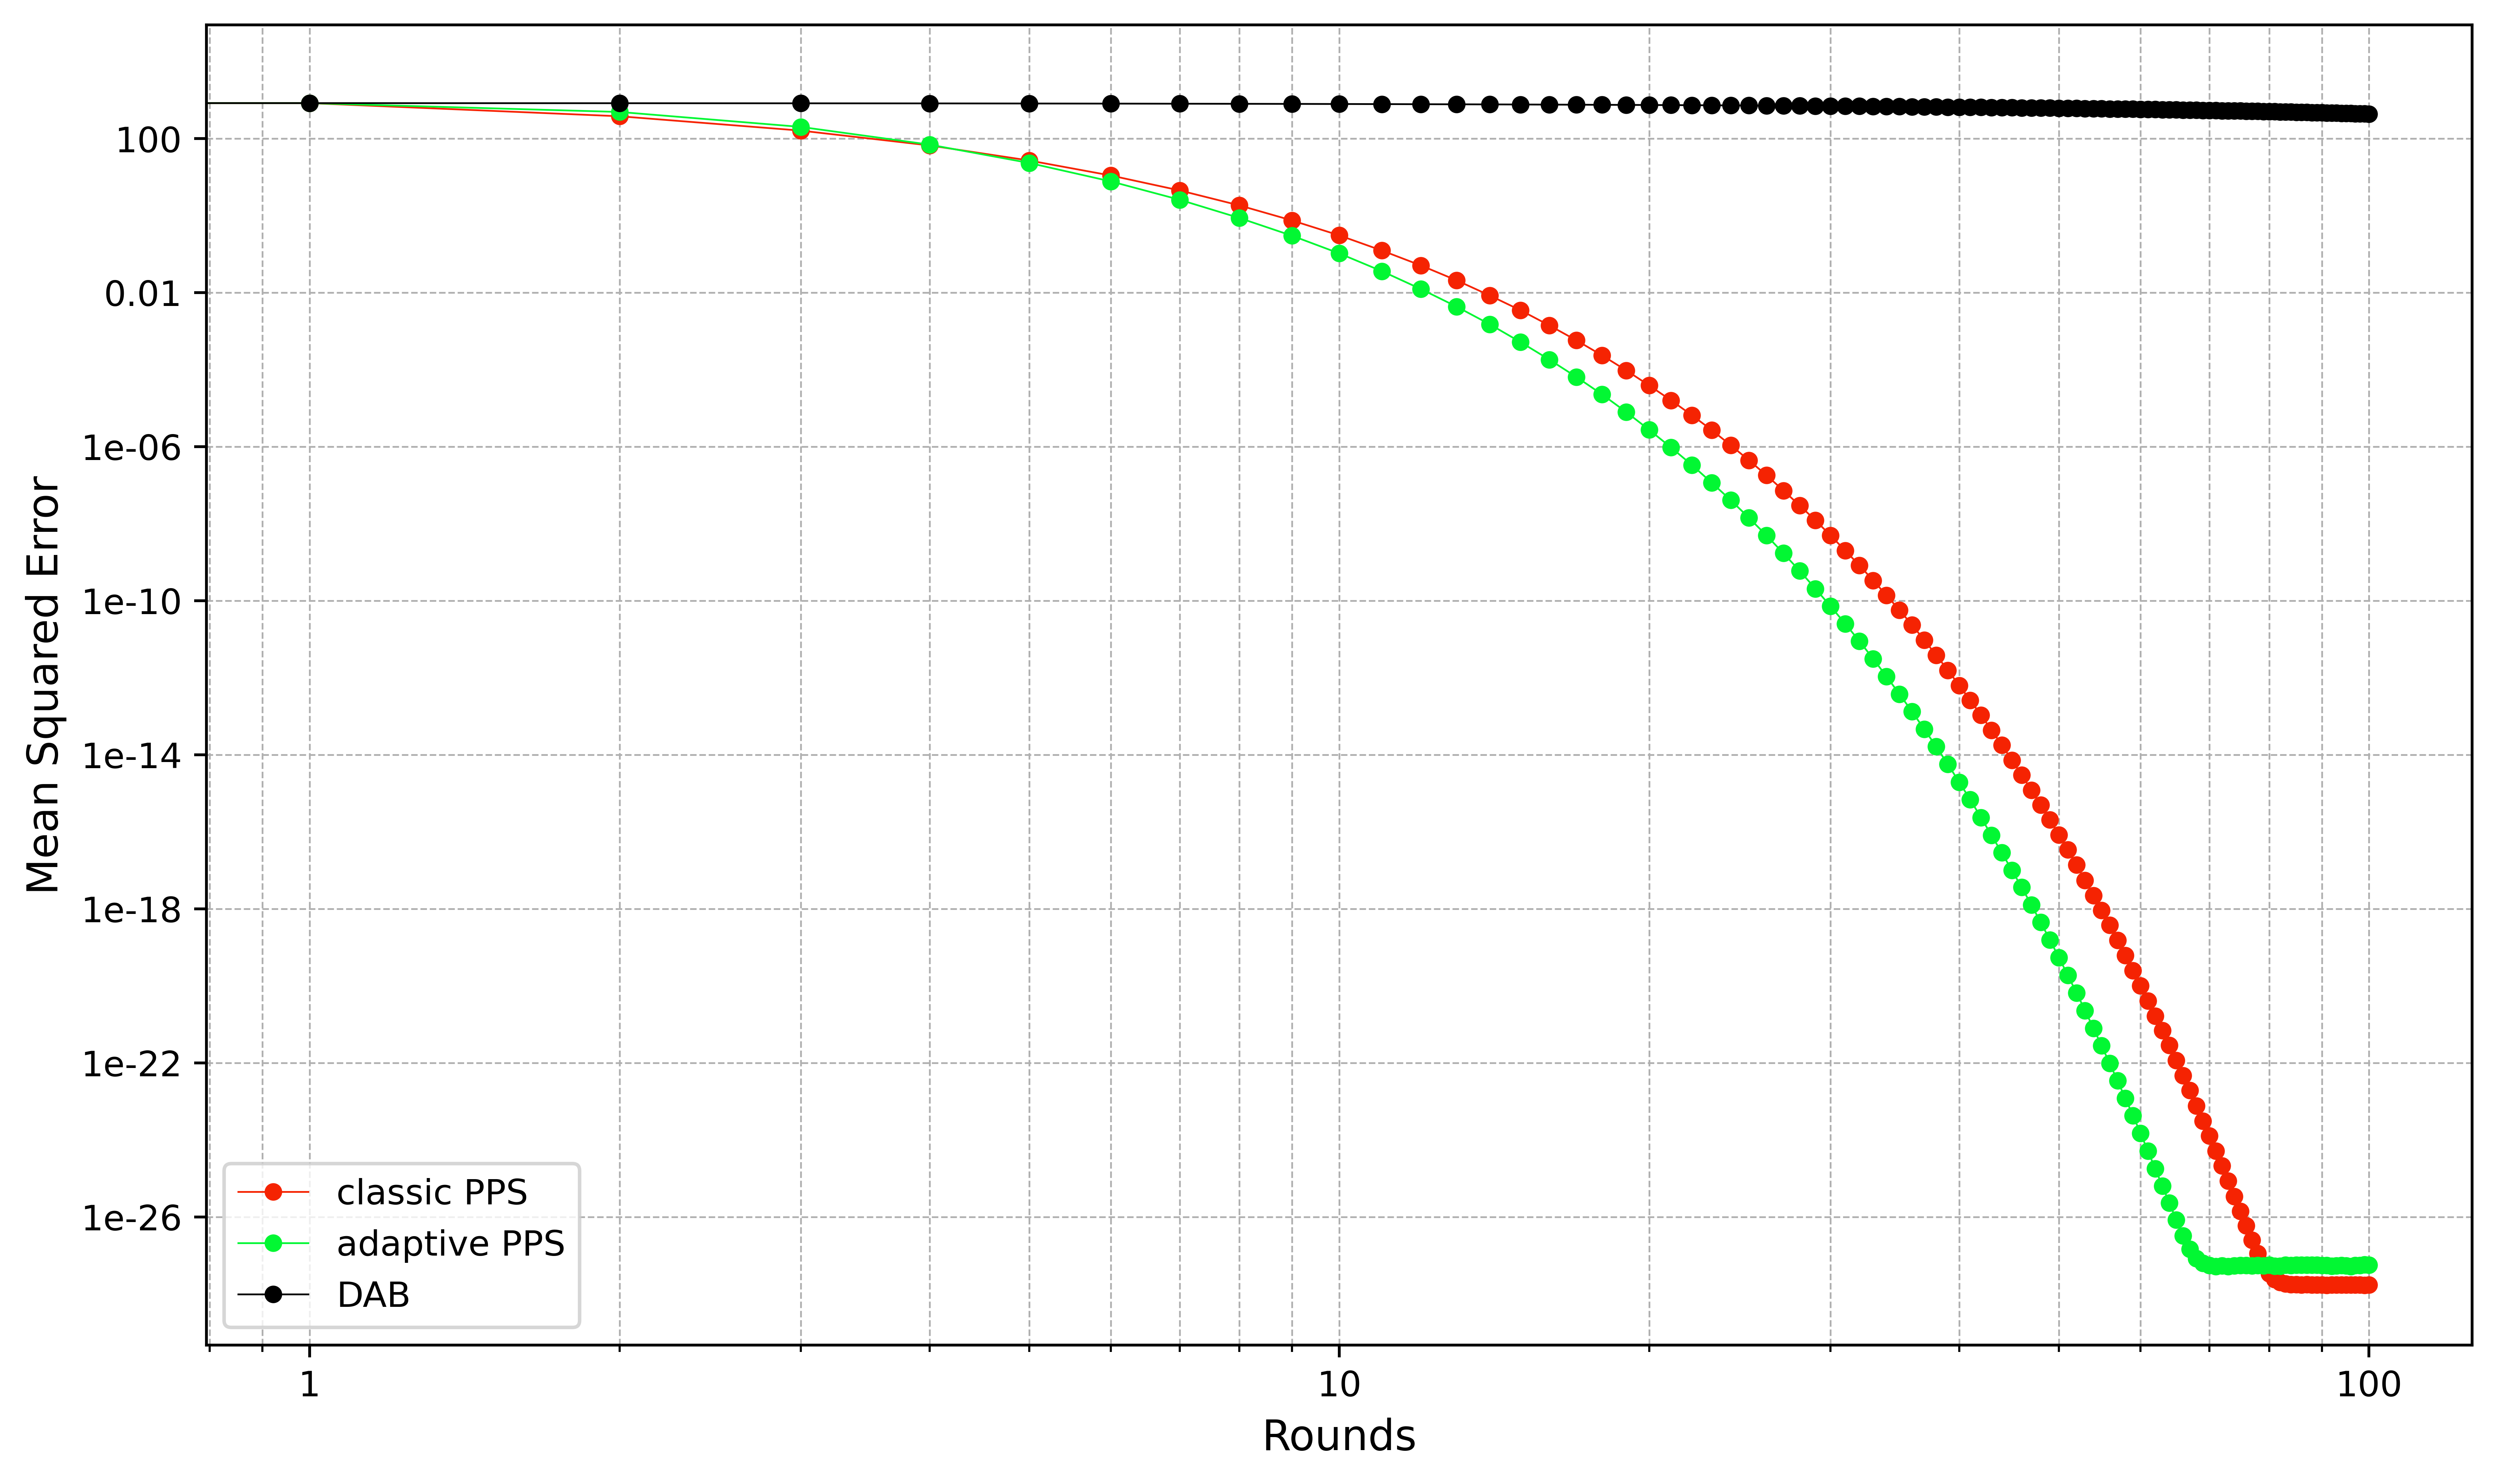
\includegraphics{figures/Simulation_outcomes/CompleteGraph/DAB_vs_PPS_CG_r100_n1024_averaged_loglog.png}}
%    \caption{Complete Graph: mean squared error per rounds (log-log)}
%    \label{fig:completegraphMSEperRoundLogLog}
%\end{figure}

\textbf{Deterministic Agreement-Based Algorithm (DAB)}: One can observe that the black line shows constant mean squared error reduction, indicating that this algorithm does not improve the load balance by much over time. The DAB performs poorly due to the rigid determinism; DAB uses a fixed, deterministic load redistribution rule, where one node looks for the minimal loaded neighbor and proposes to that node. Since for the complete graph each node are interconnected, the neighbors with the minimal loads are the same for every node. Thus, the deterministic strategy proposing to the minimal neighbor does not distribute load in suboptimal ways. The number of load transfers in this scenario per round is very limited, resulting in poor mean squared error reduction. The main observation is that deterministic methods can struggle in high-connectivity environments because they fail to exploit randomness or adaptivity. Figure \ref{fig:dabCompleteModelFit} shows the exponential regression fit for the MSE data when the DAB algorithm as a load balancing algorithm is applied to the network. The fitted curve is expressed by the equation $MSE=844.63*e^{-0.01}*r$. The decay rate of -0.01 suggests a very slow decrease in MSE. The fitted curve and model seem very suitable for the MSE data, since the fitted curve aligns with the MSE data. In summary, the exponential regression model captures the slow and steady MSE reduction of DAB over rounds, highlighting its slow but consistent convergence behavior.

%\begin{figure}[H]
%    \centering
%    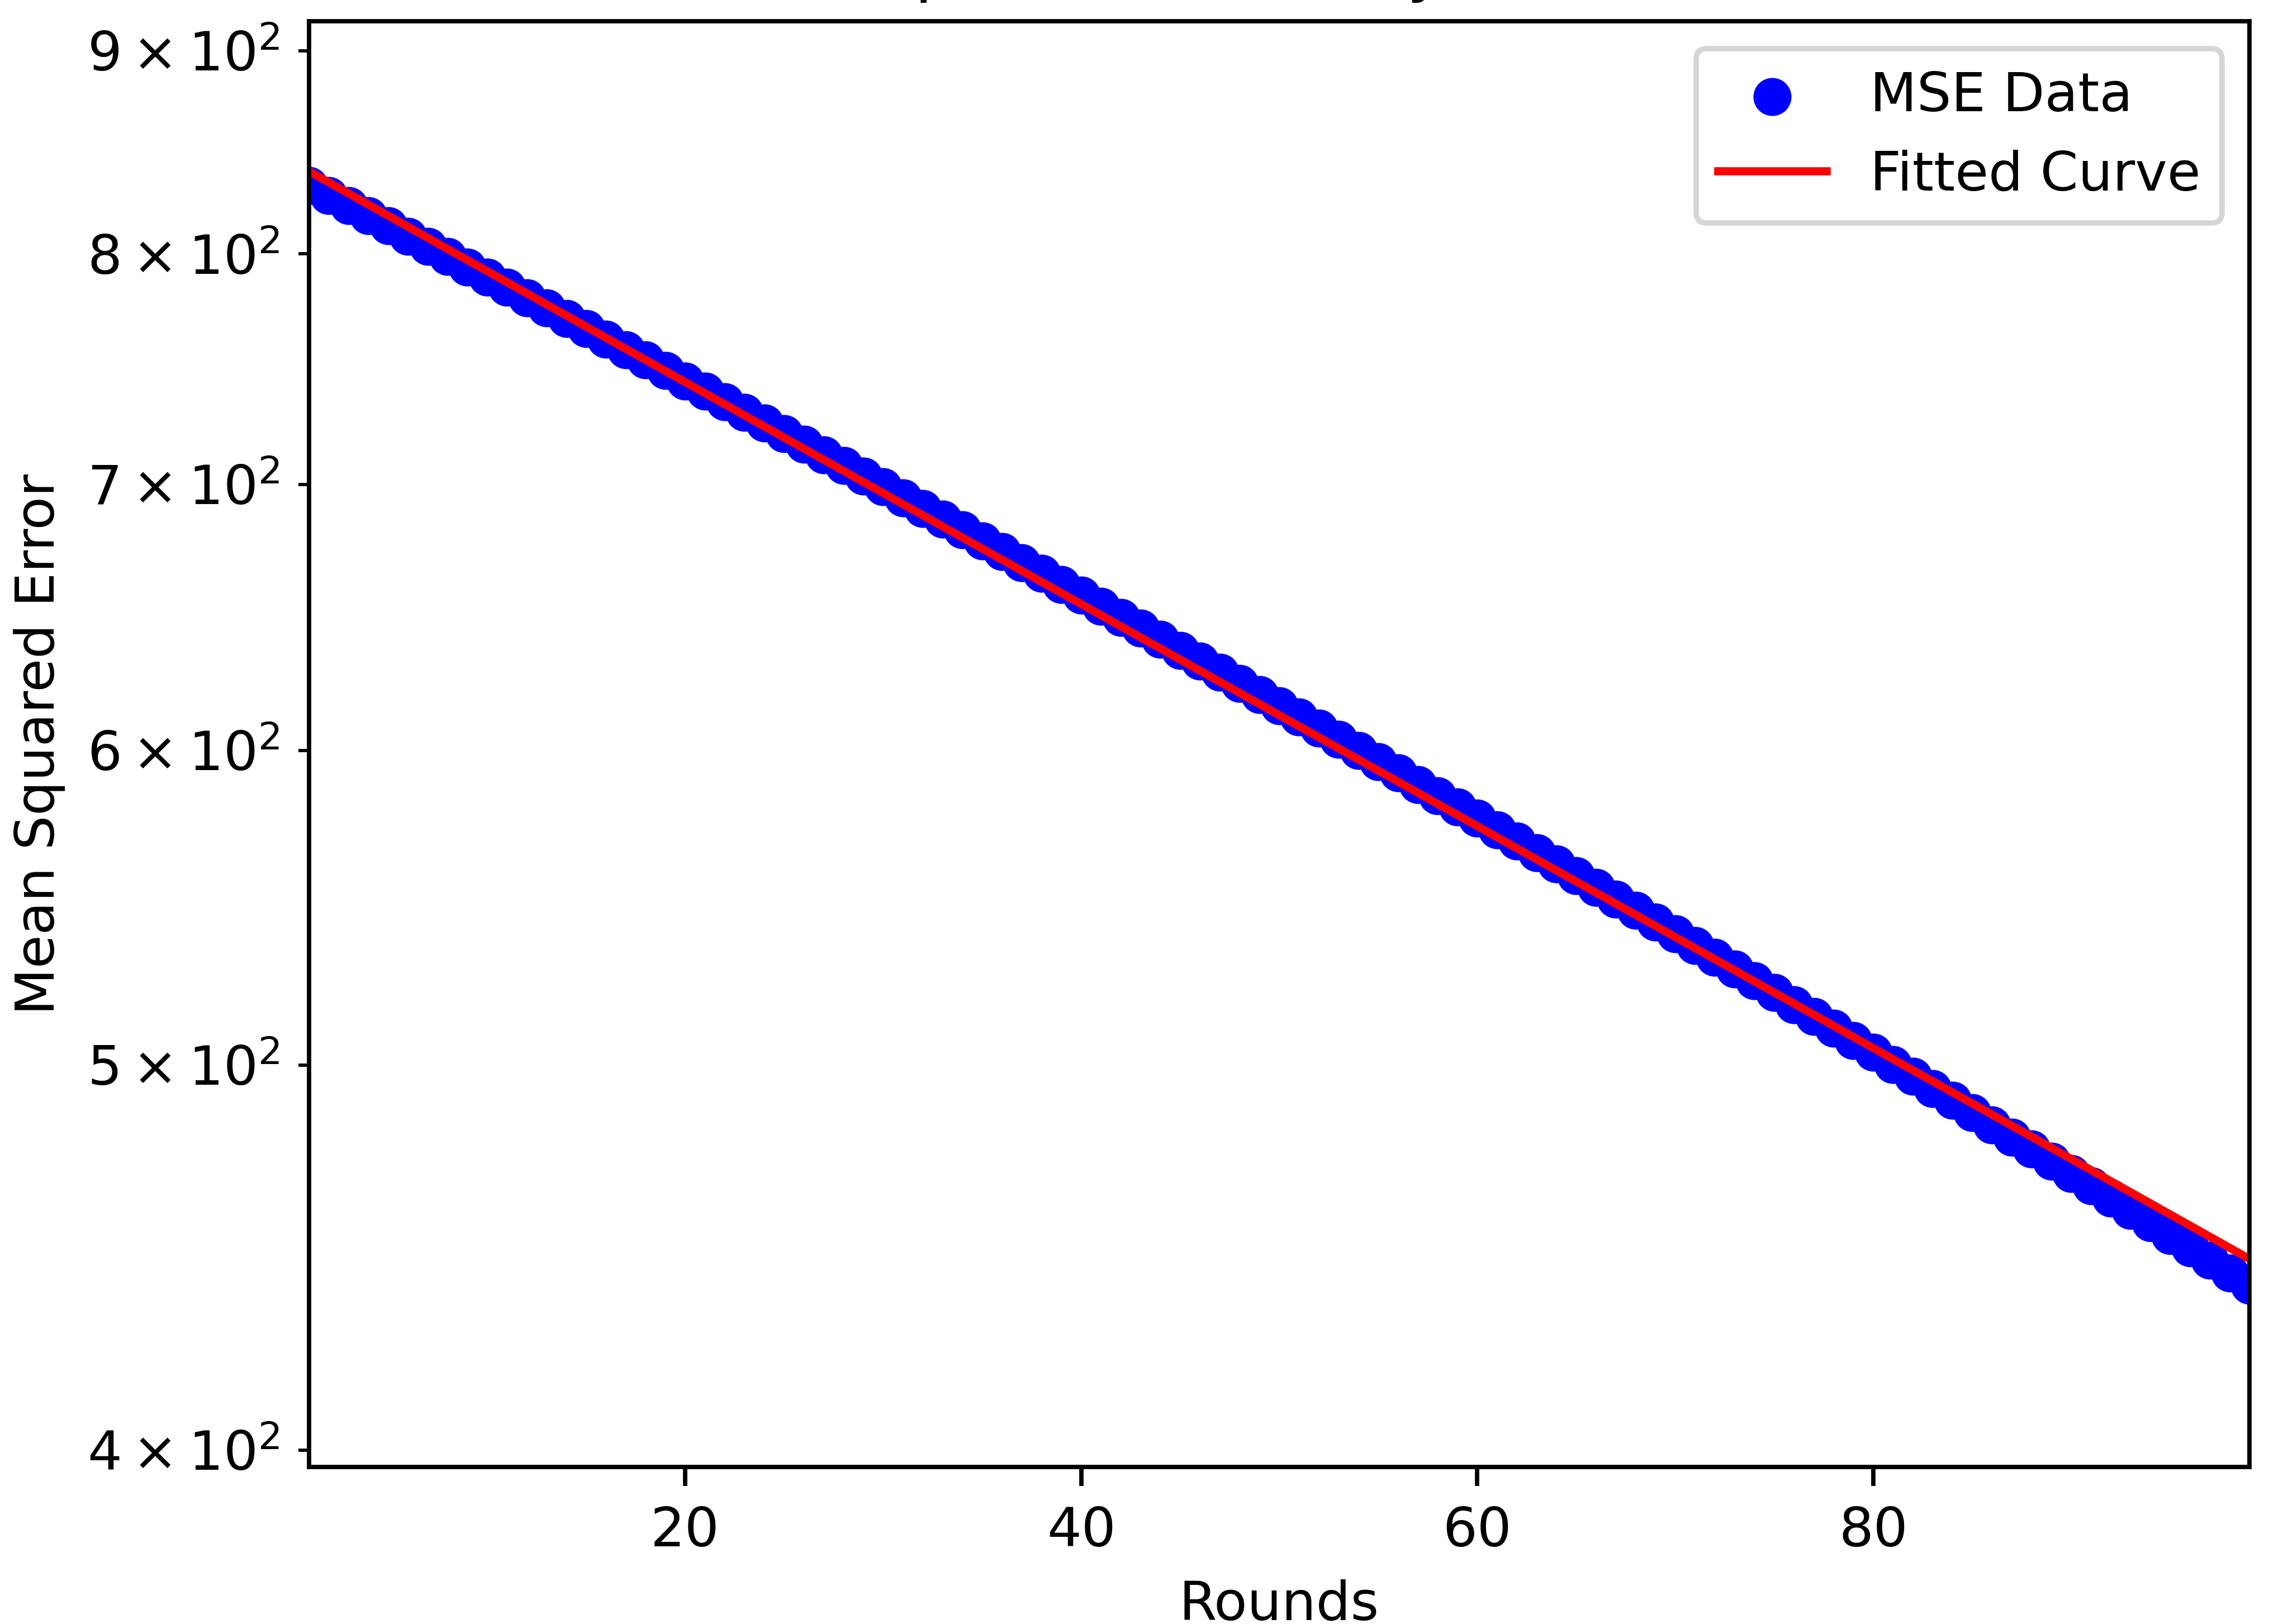
\includegraphics[width=\linewidth]{figures/Simulation_outcomes/CompleteGraph/DAB/DAB_modelfitting_rounds_99_model_1.png}
%    \caption{Exponential Decay Fit: DAB}
%    \label{fig:dabCompleteModelFit}
%\end{figure}

\textbf{Push-Pull Sum algorithm (PPS)}: The PPS-curve decreases gradually in mean squared error, showing significant error reduction over time. Since all nodes are equally connected, no structural constraints slow down the process of pushing and pulling load from neighbors. Over time, repeated randomized exchanges smooth out load imbalances, leading to a exponential decay in mean squared error. Classic PPS does not differentiate between "highly imbalanced" and "near-balanced" nodes. Load transfers happen uniformly, even when the system is close to equilibrium, which slows convergence in later rounds. Figure \ref{fig:ppsCompleteModelFit} visualizes the MSE data of the PPS load balancing algorithm, plotted for the rounds 10 to 80 and fitted with the exponential regression model. The best-fit follows the equation $MSE=2530.41*e^{-0.9*r}$. The graph uses a logarithmic scale for the mean squared error. The fitted curve aligns closely with the MSE data, so the exponential model accurately describes the behaviour of the algorithm for this region. The decay rate of -0.9 indicates a steep decrease in MSE. This suggests that the PPS load balancing algorithm reduces the MSE in a exponential way.

%\begin{figure}[H]
%    \centering
%    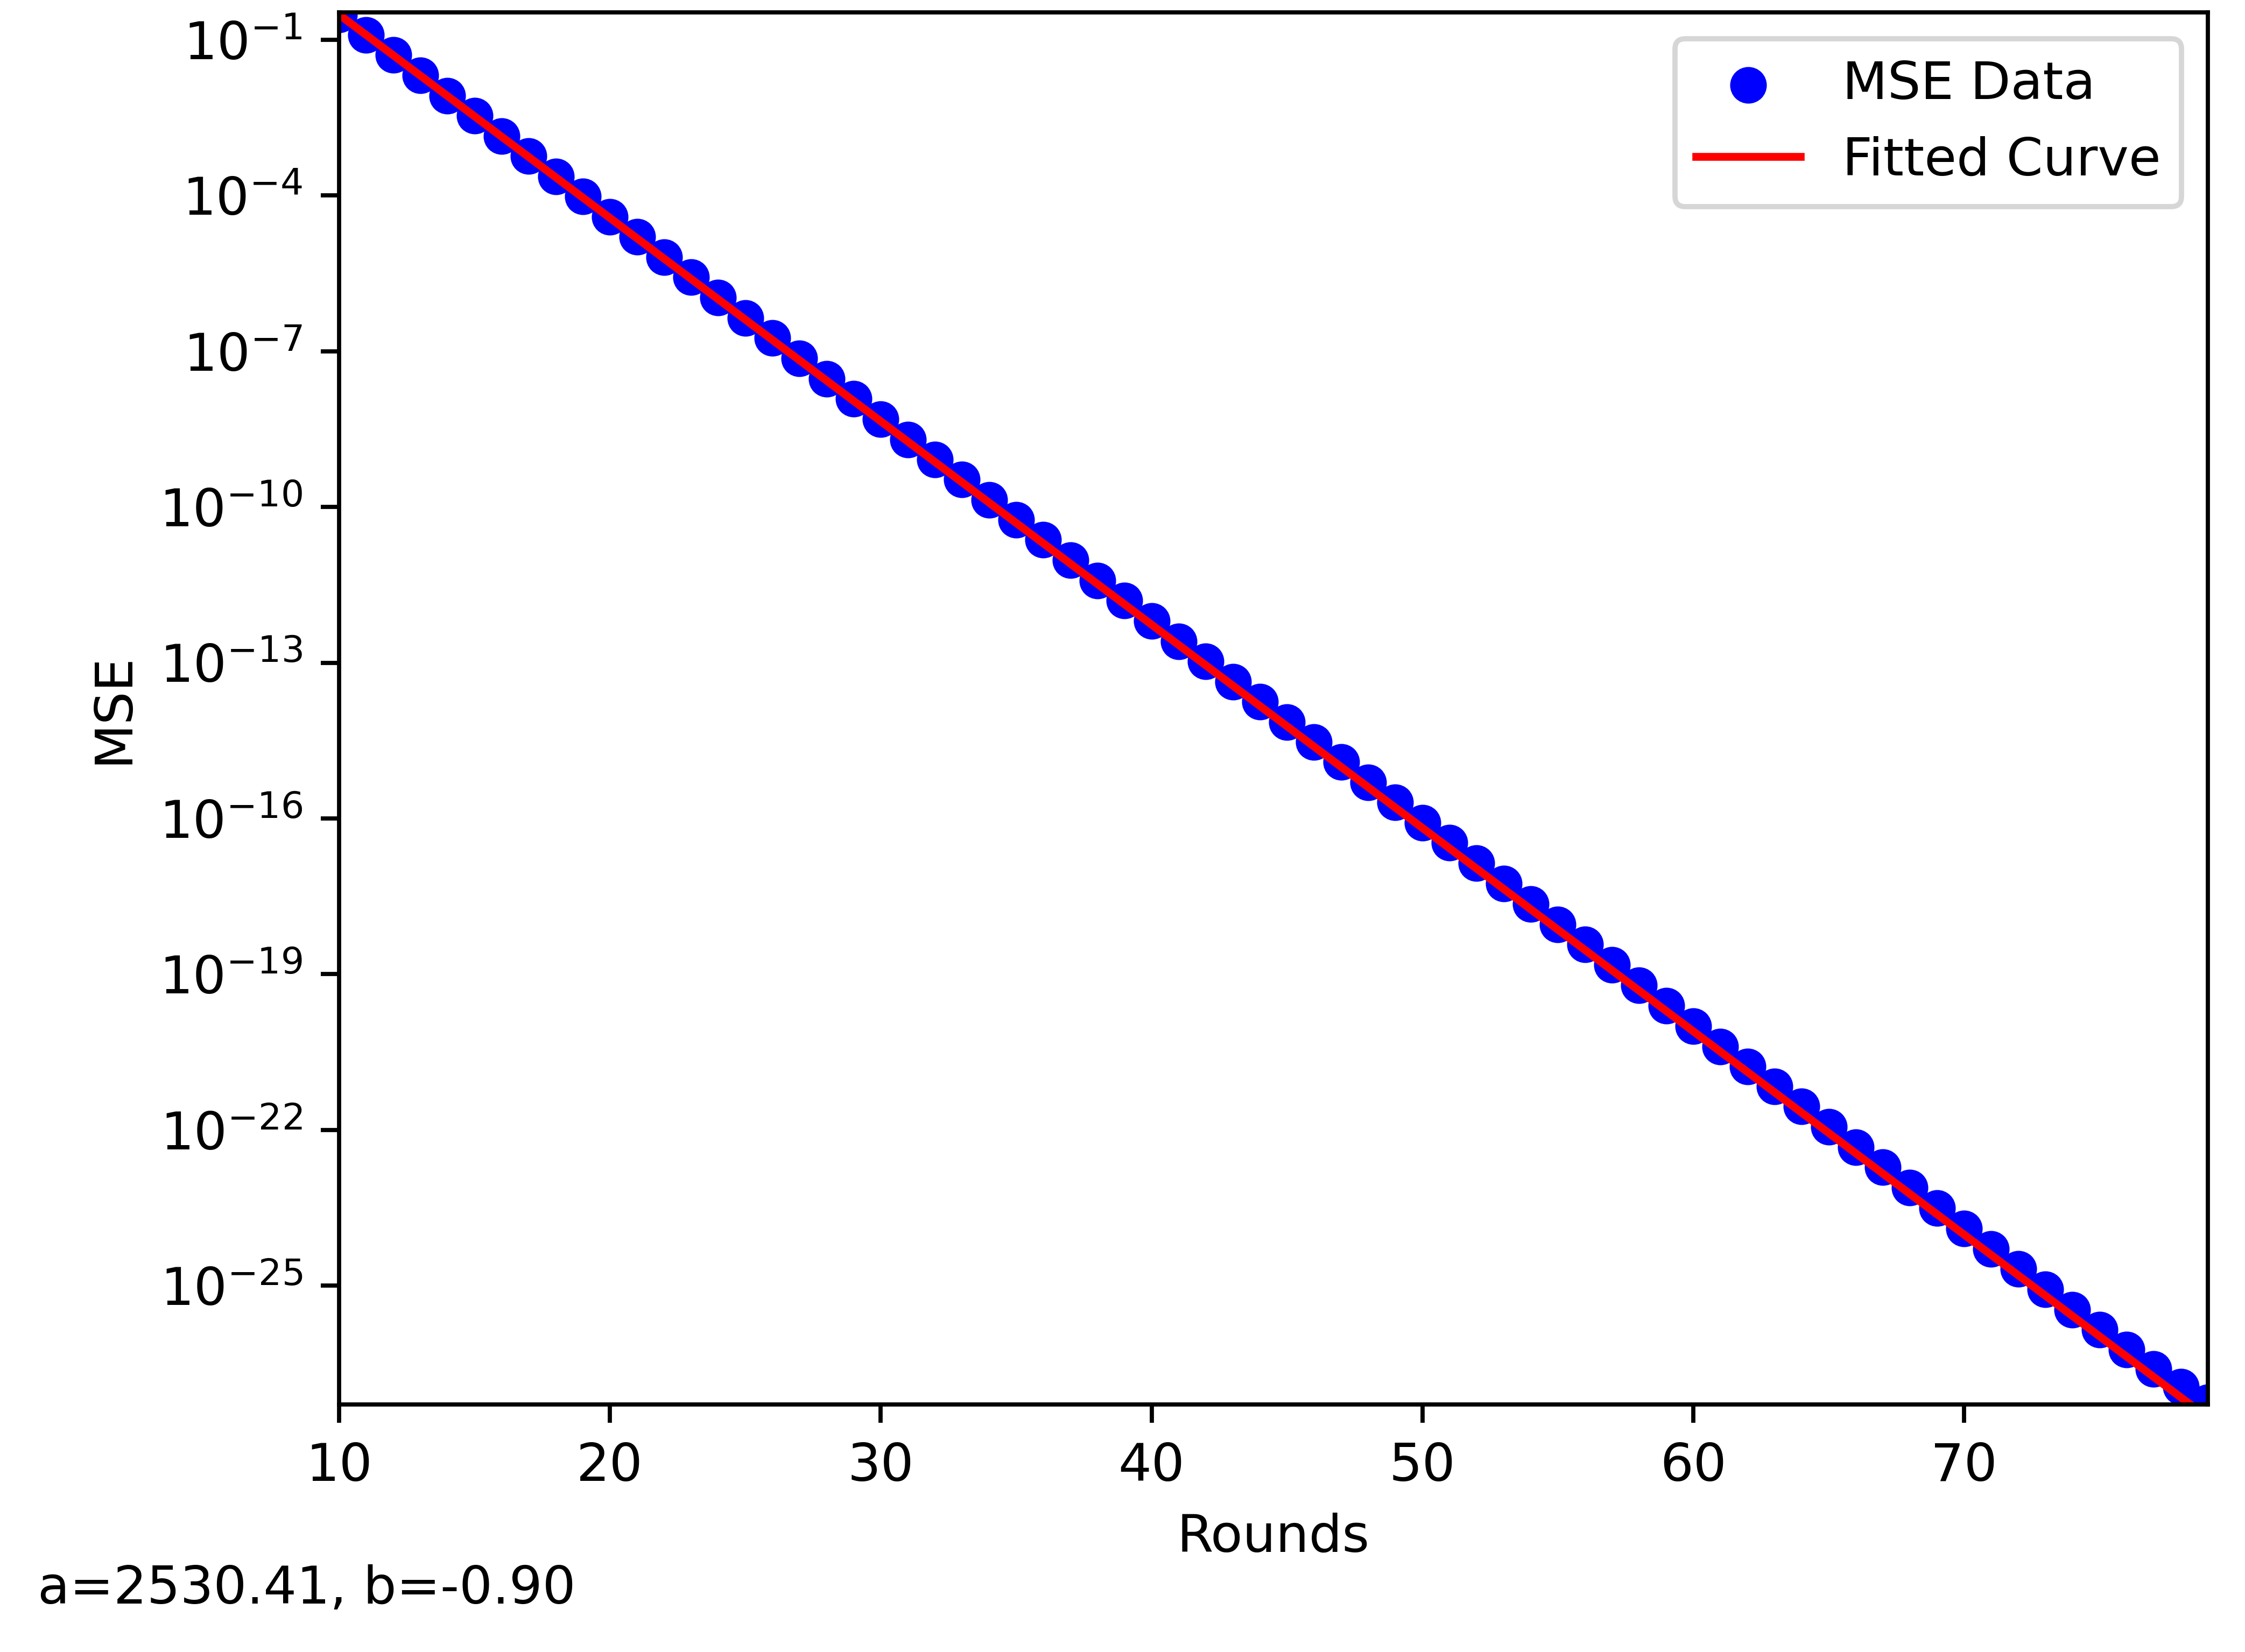
\includegraphics[width=\linewidth]{figures/Simulation_outcomes/CompleteGraph/PPS/PPS_modelfitting_rounds_79_model_1.png}
%    \caption{Exponential Decay Fit: PPS}
%    \label{fig:ppsCompleteModelFit}
%\end{figure}

\textbf{Adaptive Push-Pull Algorithm (ATPPS)}: The ATPPS-curve decreases faster than the red curve, reaching lower MSE values earlier. Adaptive Thresholding: Nodes adaptively decide when and how much load to exchange based on thresholds. For example: Nodes with significantly higher load push more load to neighbors. Nodes closer to balance reduce their interactions. Adaptive strategies reduce redundant exchanges when the system is near equilibrium, focusing resources on nodes with the largest imbalance. In a complete graph, adaptive decisions propagate quickly because every node can directly communicate with others. The adaptive mechanism leverages the symmetry and high connectivity of the complete graph to reduce MSE more quickly and efficiently. In Figure \ref{fig:atppsCompleteModelFit} the exponential regression fit is visualized for the MSE data of the ATPPS load balancing algorithm graph in the complete graph for the rounds 10 to 65. The fitted curve is expressed by the equation $MSE=4309.94*e^{-1.06}*r$. A steep error reduction is indicated by the decay rate of -1.06. As the PPS algorithm the ATPPS algorithm reduces the error very effectively in an exponential manner. Rounds 66 to 100 show a plateauing of the MSE data.

%\begin{figure}[H]
%    \centering
%    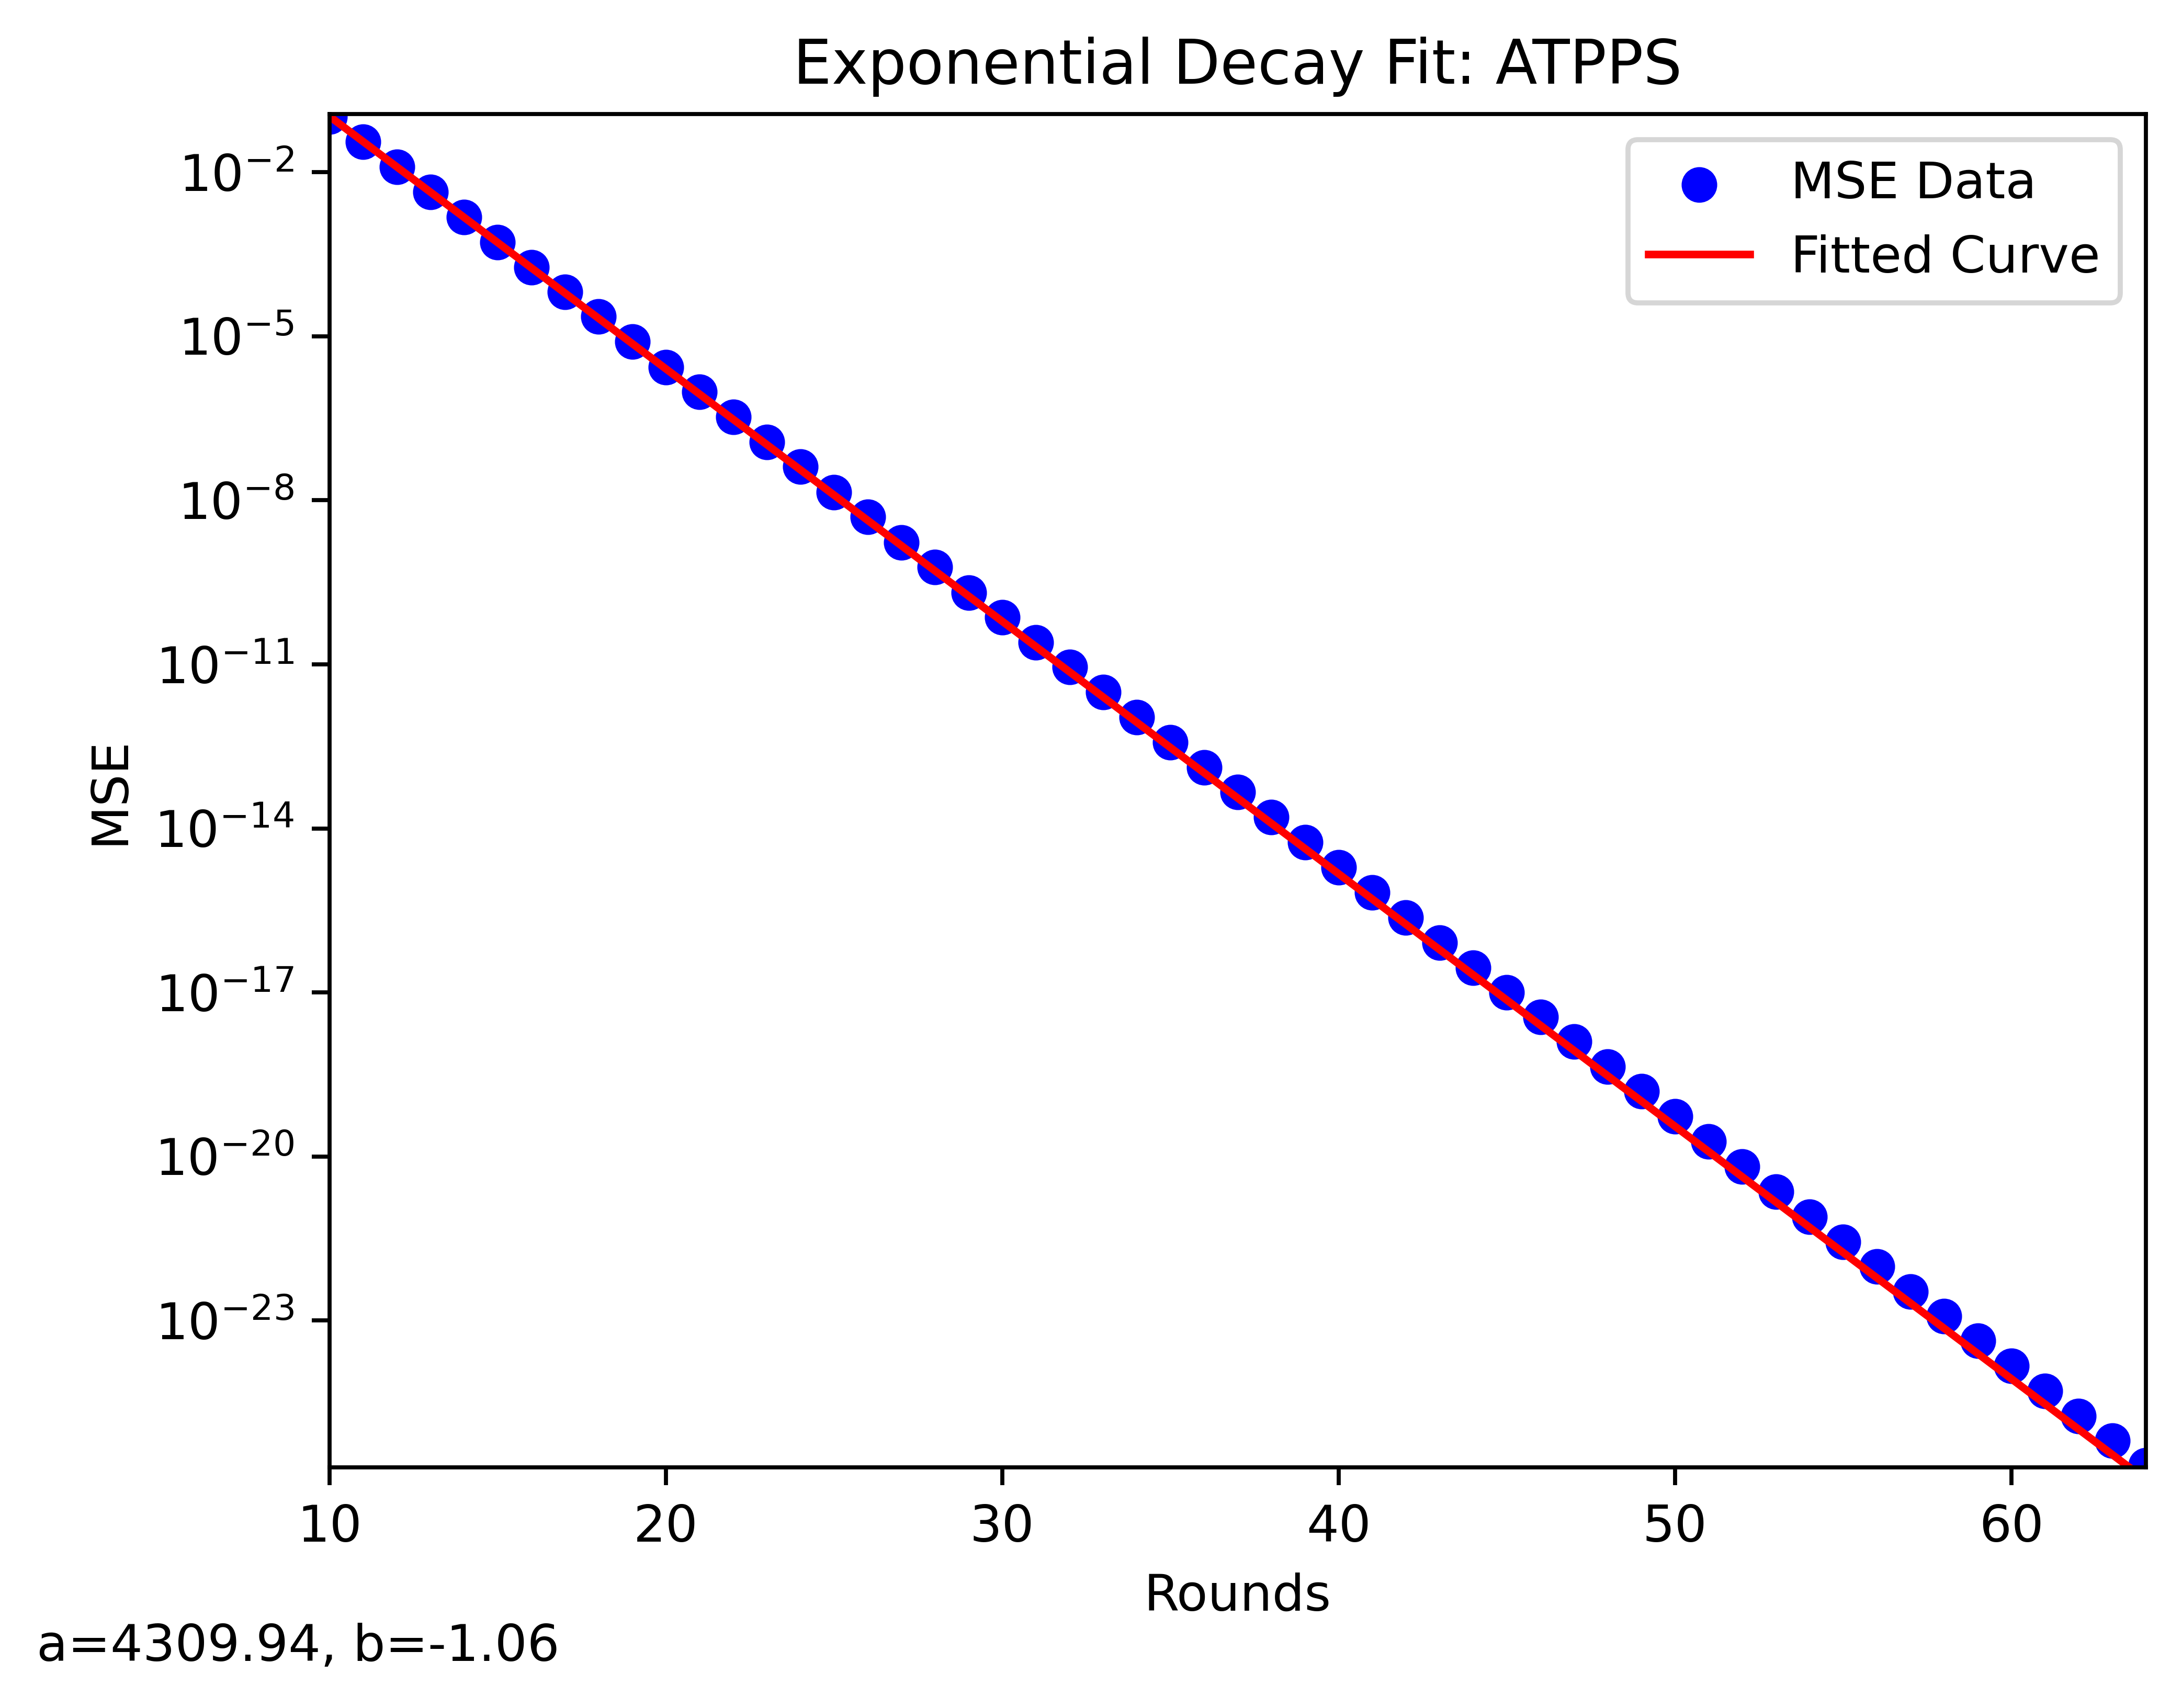
\includegraphics[width=\linewidth]{figures/Simulation_outcomes/CompleteGraph/ATPPS/ATPPS_modelfitting_rounds_64_model_1.png}
%    \caption{Exponential Decay Fit: ATPPS}
%    \label{fig:atppsCompleteModelFit}
%\end{figure}

Figure \ref{fig:completegrapslopes} visualizes a heat map of the slopes (rates of change) for the three load balancing algorithms across different regions of the graph. The values reflect how steeply the mean squared error decreases over rounds. PPS and ATPPS have steep negative slopes in the start region, namely the rounds 1-10 with a value of -92, indicating rapid initial improvement. However, their slopes in the middle (rounds 11-65) and end regions (rounds 66-100) approach zero, suggesting a plateau in performance. DAB has shallower negative slopes overall, reflecting a more gradual and consistent error reduction across all regions. The general slopes (rounds 1-100) for PPS and ATPPS (-8.4) are much steeper than DAB (-4.4), suggesting that PPS and ATPPS converge faster on average. The end region is chosen as 66-100 to catch the trend of plateauing for the ATPPS and also for PPS which is beginning to plateau in errror reduction in later rounds (round $~$80-100).

%\begin{figure}
%    \centering
%    \scalebox{0.8}{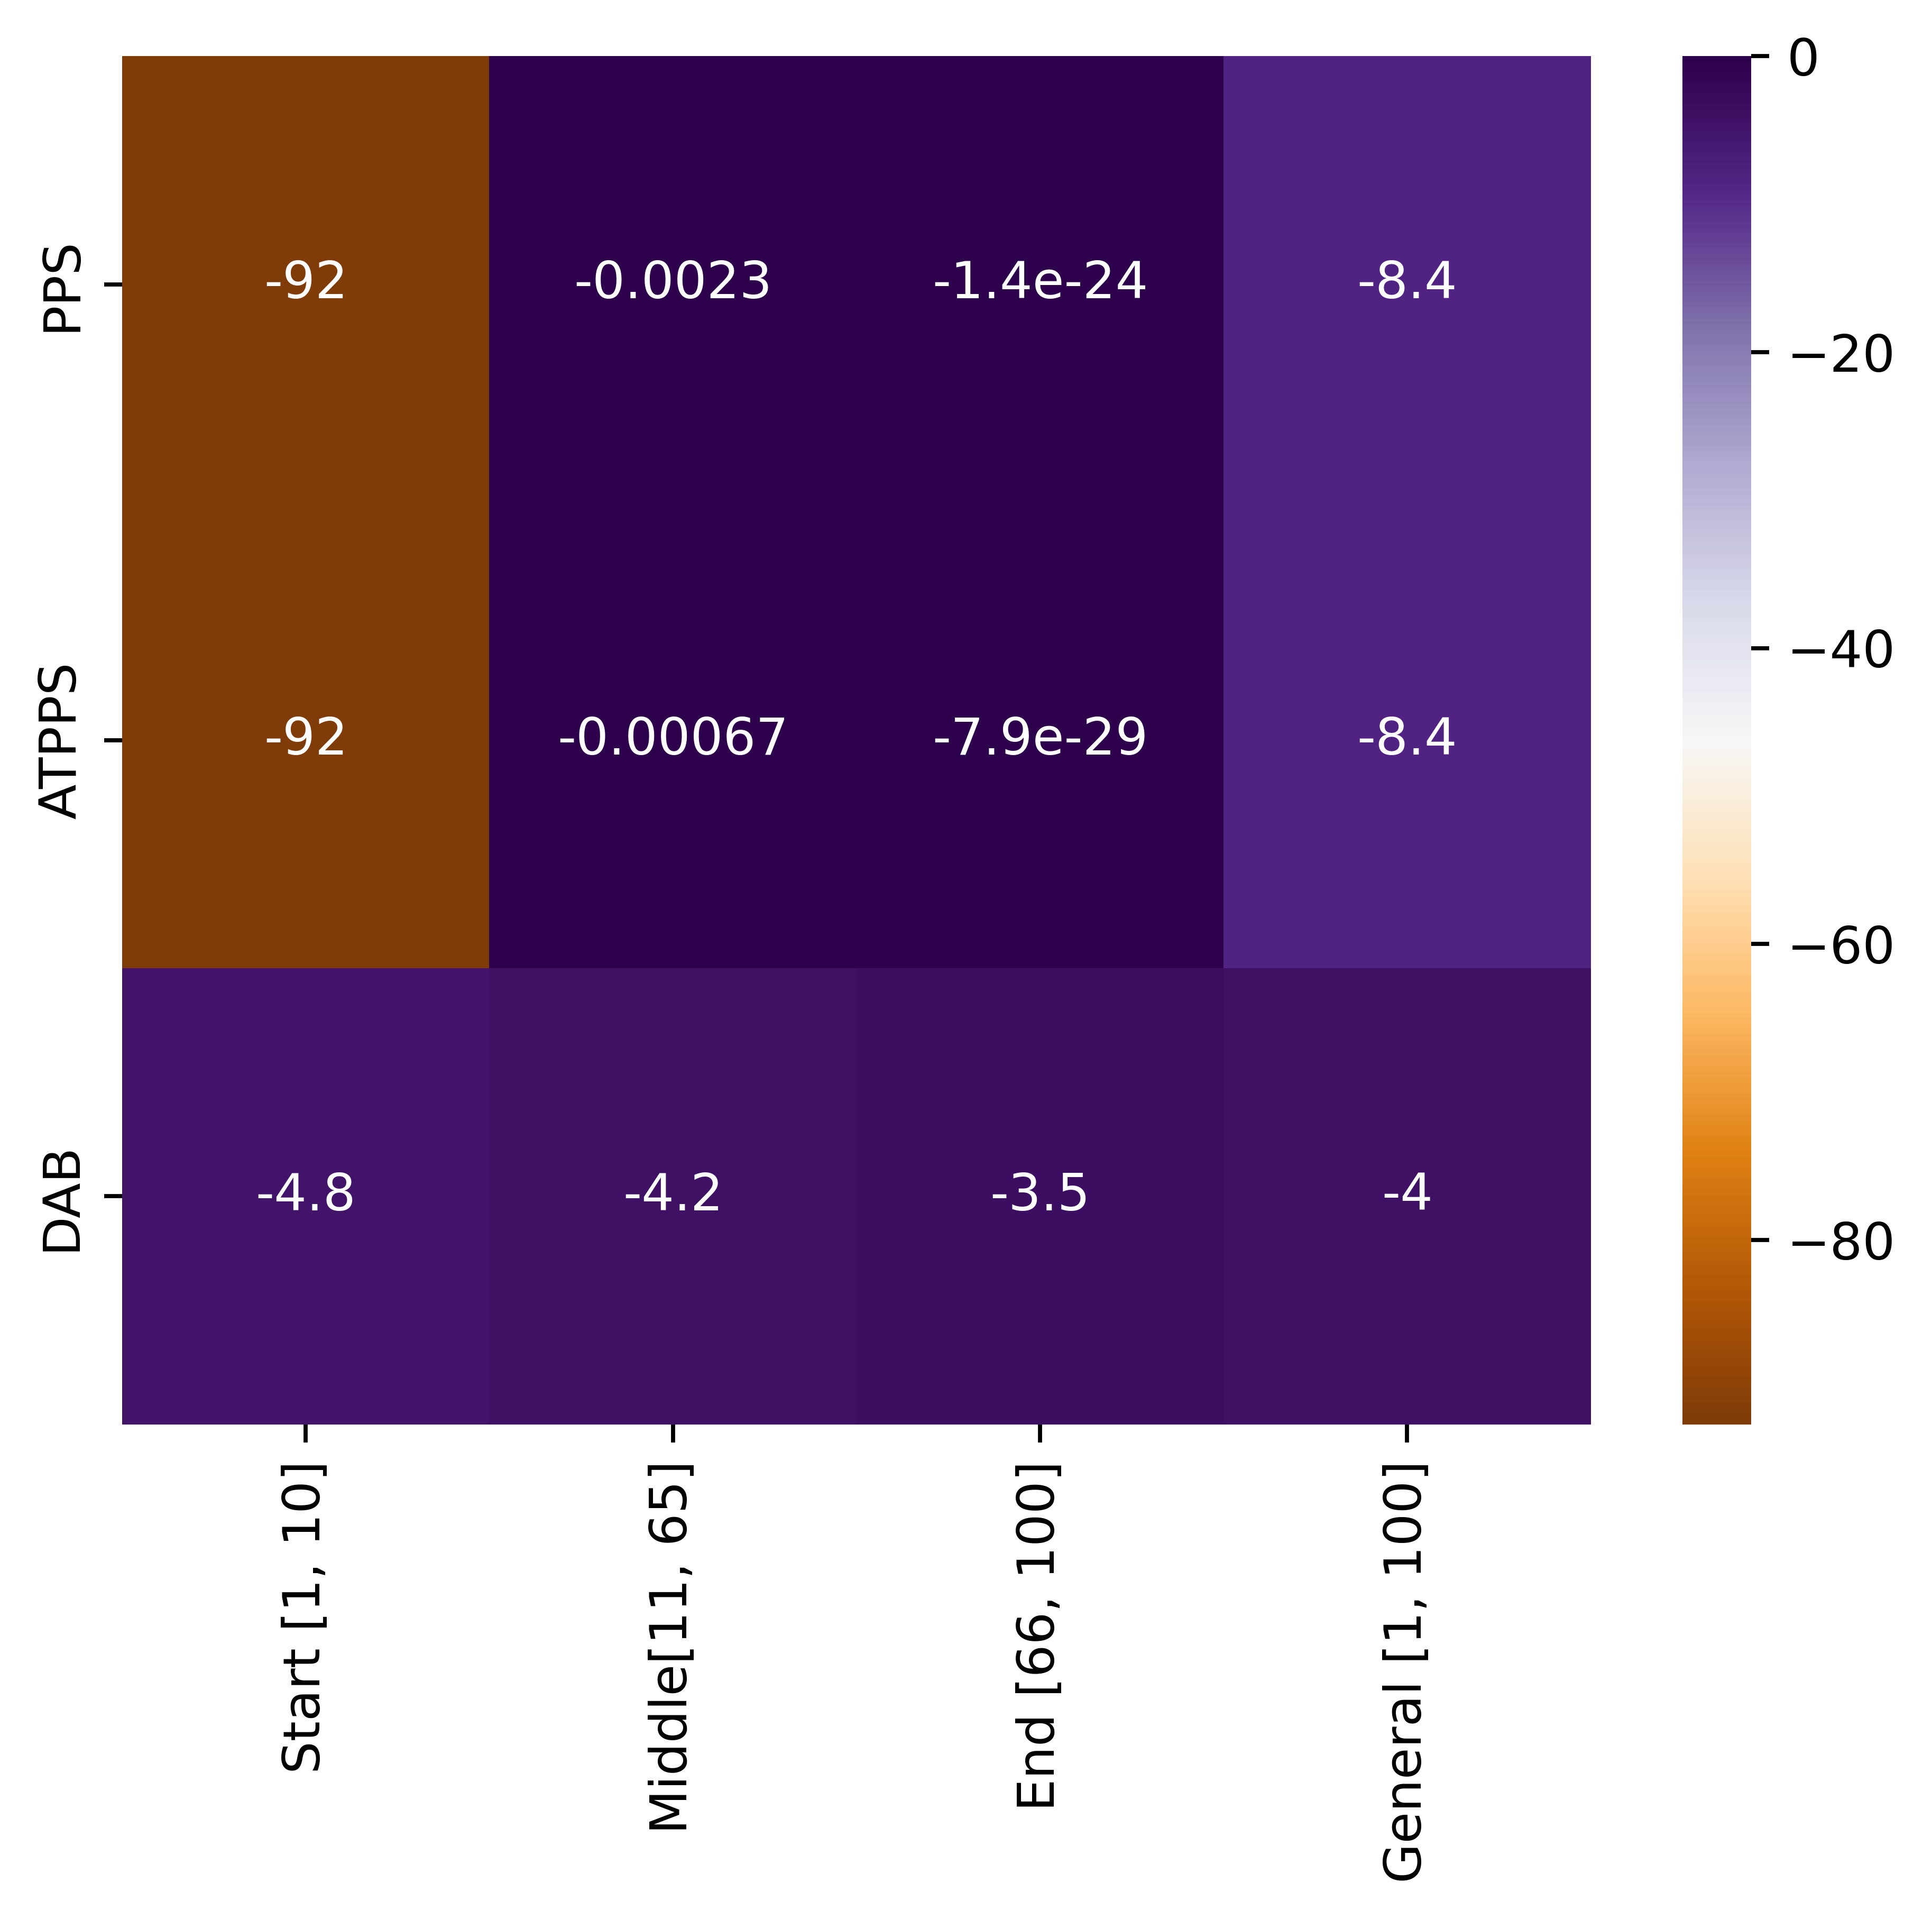
\includegraphics{figures/Simulation_outcomes/CompleteGraph/DAB_vs_PPS_vs_ATPPS_slopesheatmap_100rounds.png}}
%    \caption{Complete Graph: heat map of slopes per region}
%    \label{fig:completegrapslopes}
%\end{figure}


\section{Star Graph}\label{sec:stargraph}
For the star graph the push-pull mechanism-based protocols seem to perform well in MSE reduction, while the DAB algorithm seem to struggle with in this topology as depicted in figure \ref{fig:stargraphMSEperRoundLogLog}

% \begin{figure}[h]
%     \centering
%     \scalebox{0.5}{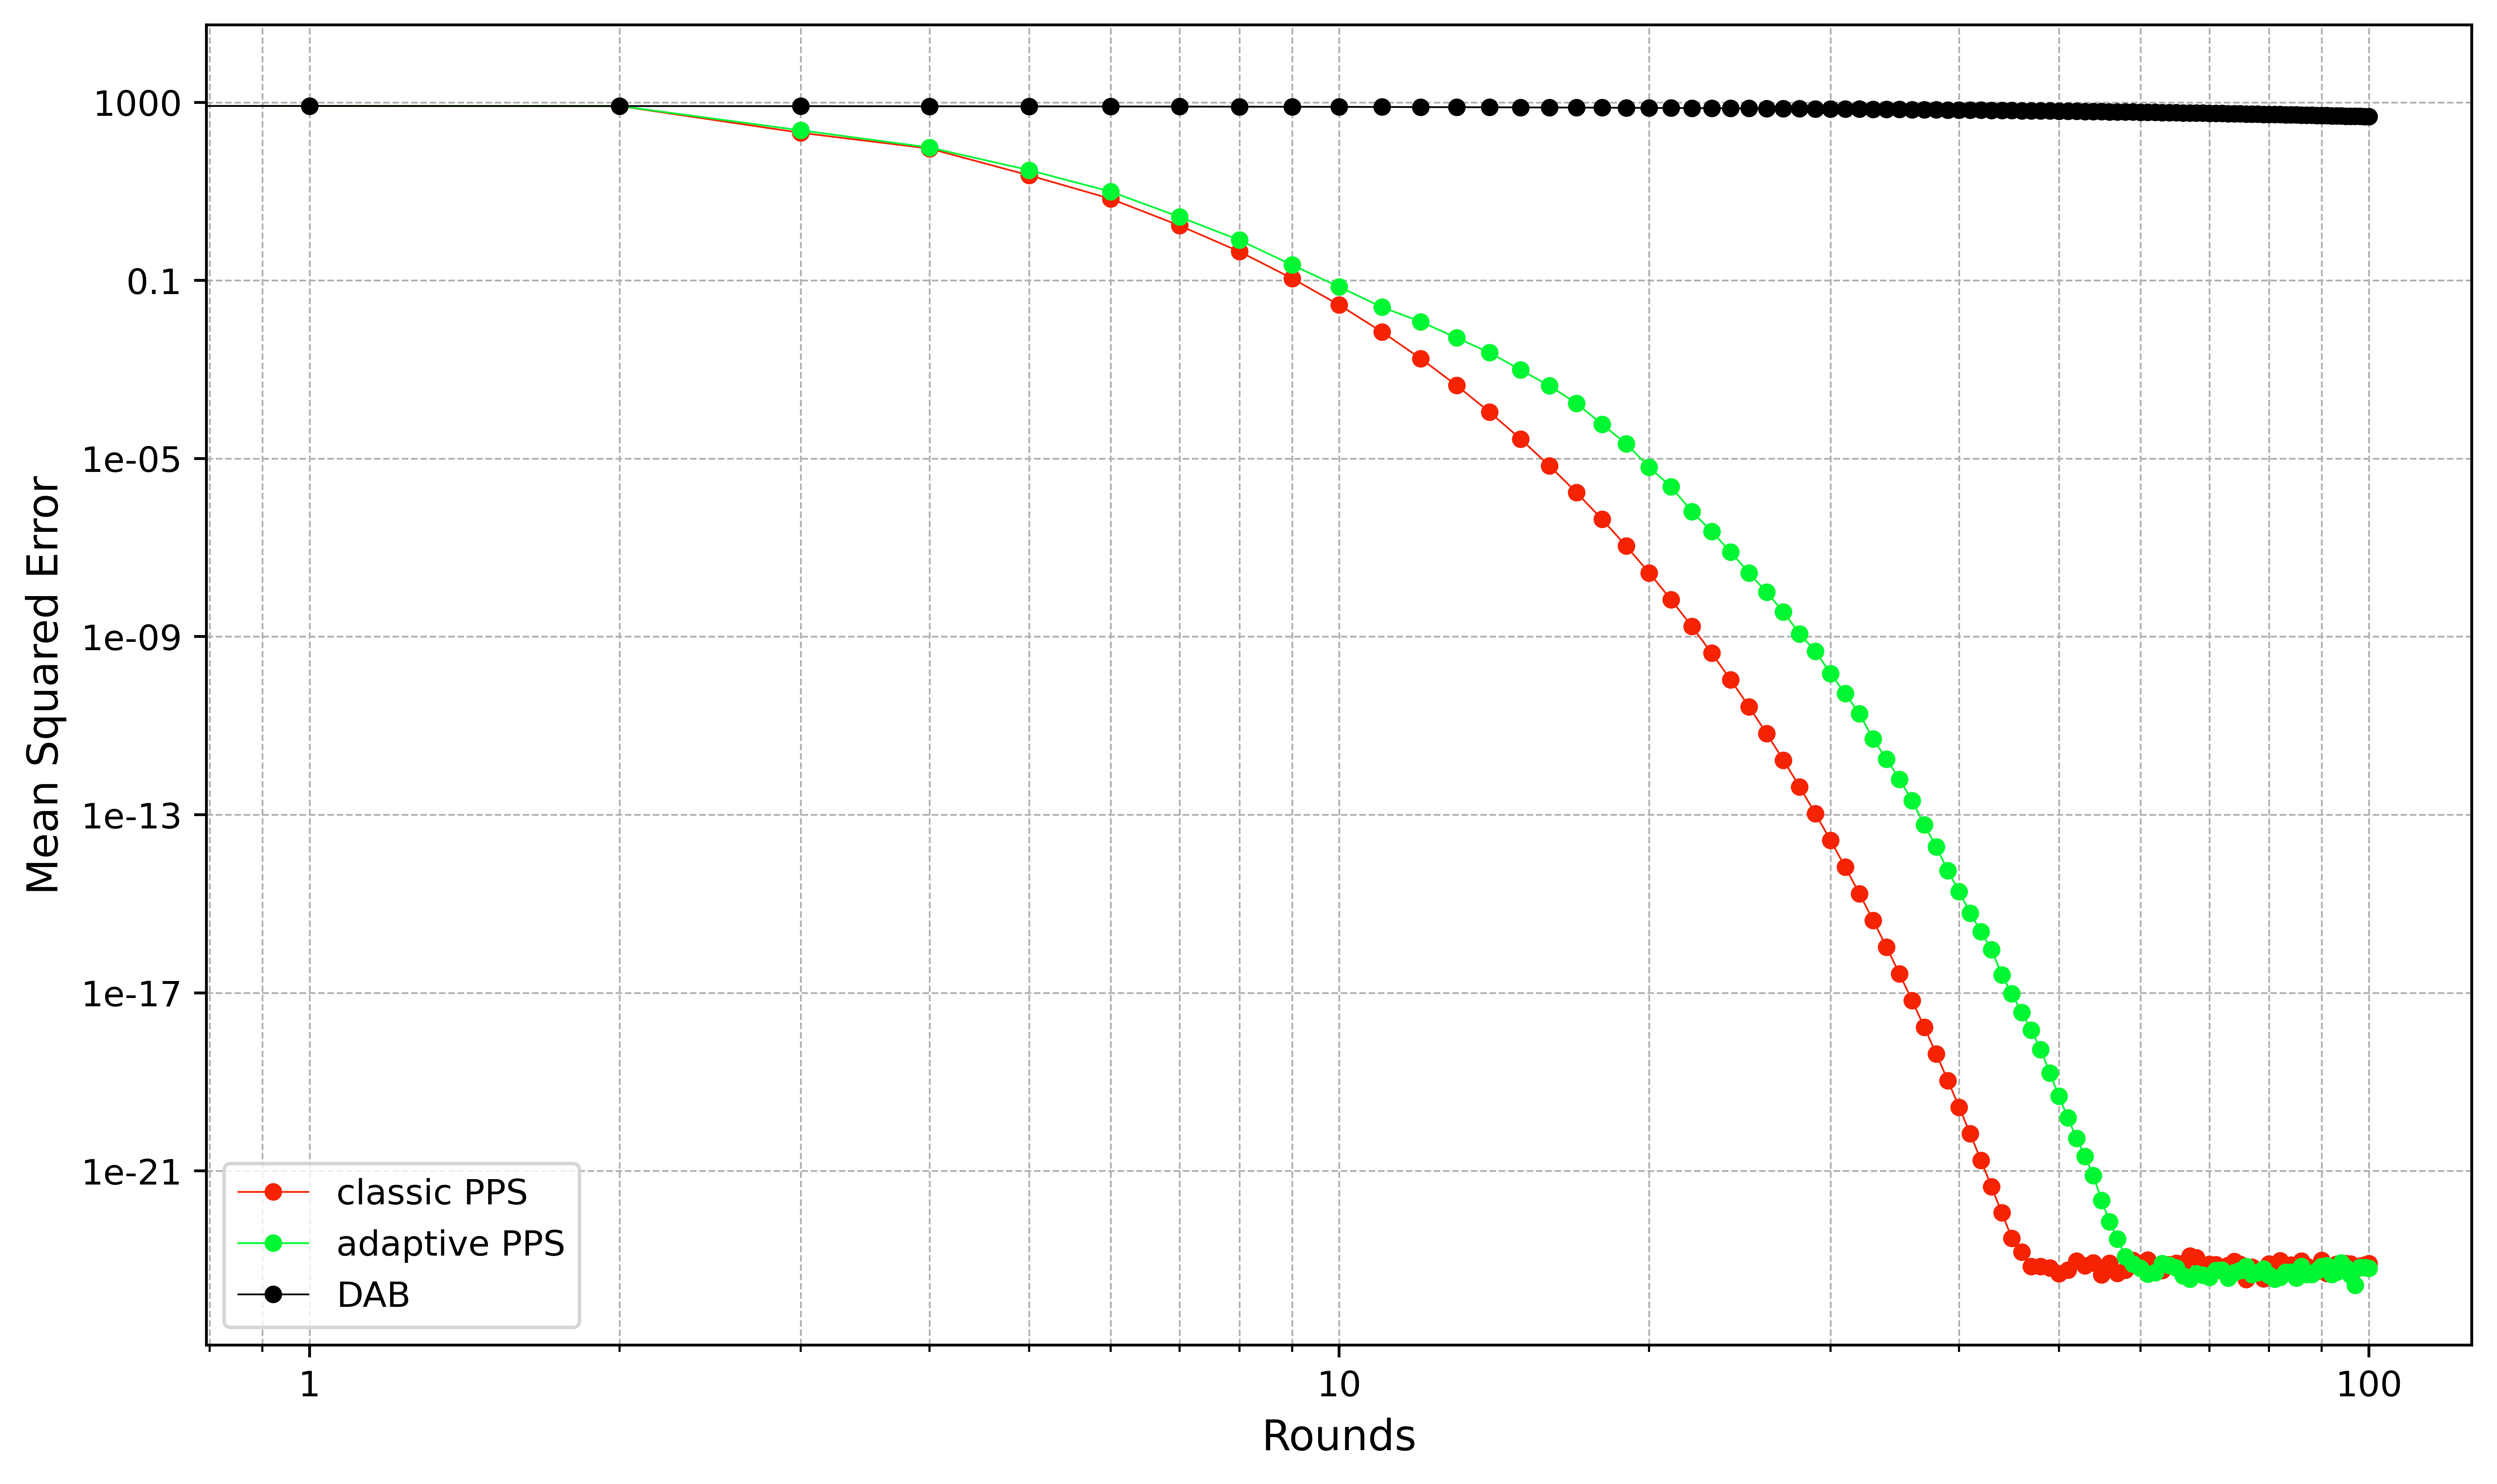
\includegraphics{figures/Simulation_outcomes/StarGraph/DAB_vs_PPS_SG_r100_n1024_averaged_loglog.png}}
%     \caption{Star Graph: mean squared error per rounds (log-log)}
%     \label{fig:stargraphMSEperRoundLogLog}
% \end{figure}

\textbf{Deal-Agreement-Based Algorithm}: DAB shows a much slower MSE reduction compared to the push-pull based algorithms, as indicated by the flatter slope of its curve. It converges minimally, with MSE remaining constant over rounds after an initial reduction. This indicates that DAB is less efficient in balancing load in a star graph topology, likely due to its deterministic nature and lack of dynamic adaptability. In the star topology all the leaves have the central node as a partner, and thus each node chooses the same node as an transfer partner. When the central node has a higher load than the leaf requesting a load transfer, than no load transfer is happening between these two nodes (bottleneck). As seen in figure \ref{fig:dabStarModelFit} the MSE data for the DAB-balanced network aligns nearly perfectly with the fitted curve of the exponential regression model with equation $MSE_r=840.42*e^{-0.01*r}$ for the rounds 1 to 100, eventhough the decay rate of -0.01 indicates a very slow decay. From round to round the improvement in the network is significantly minimal and thus highlights the inability of the DAB load balancing algorithm to balance the network within 100 rounds to a satisfying magnitude.

% \begin{figure}[H]
%     \centering
%     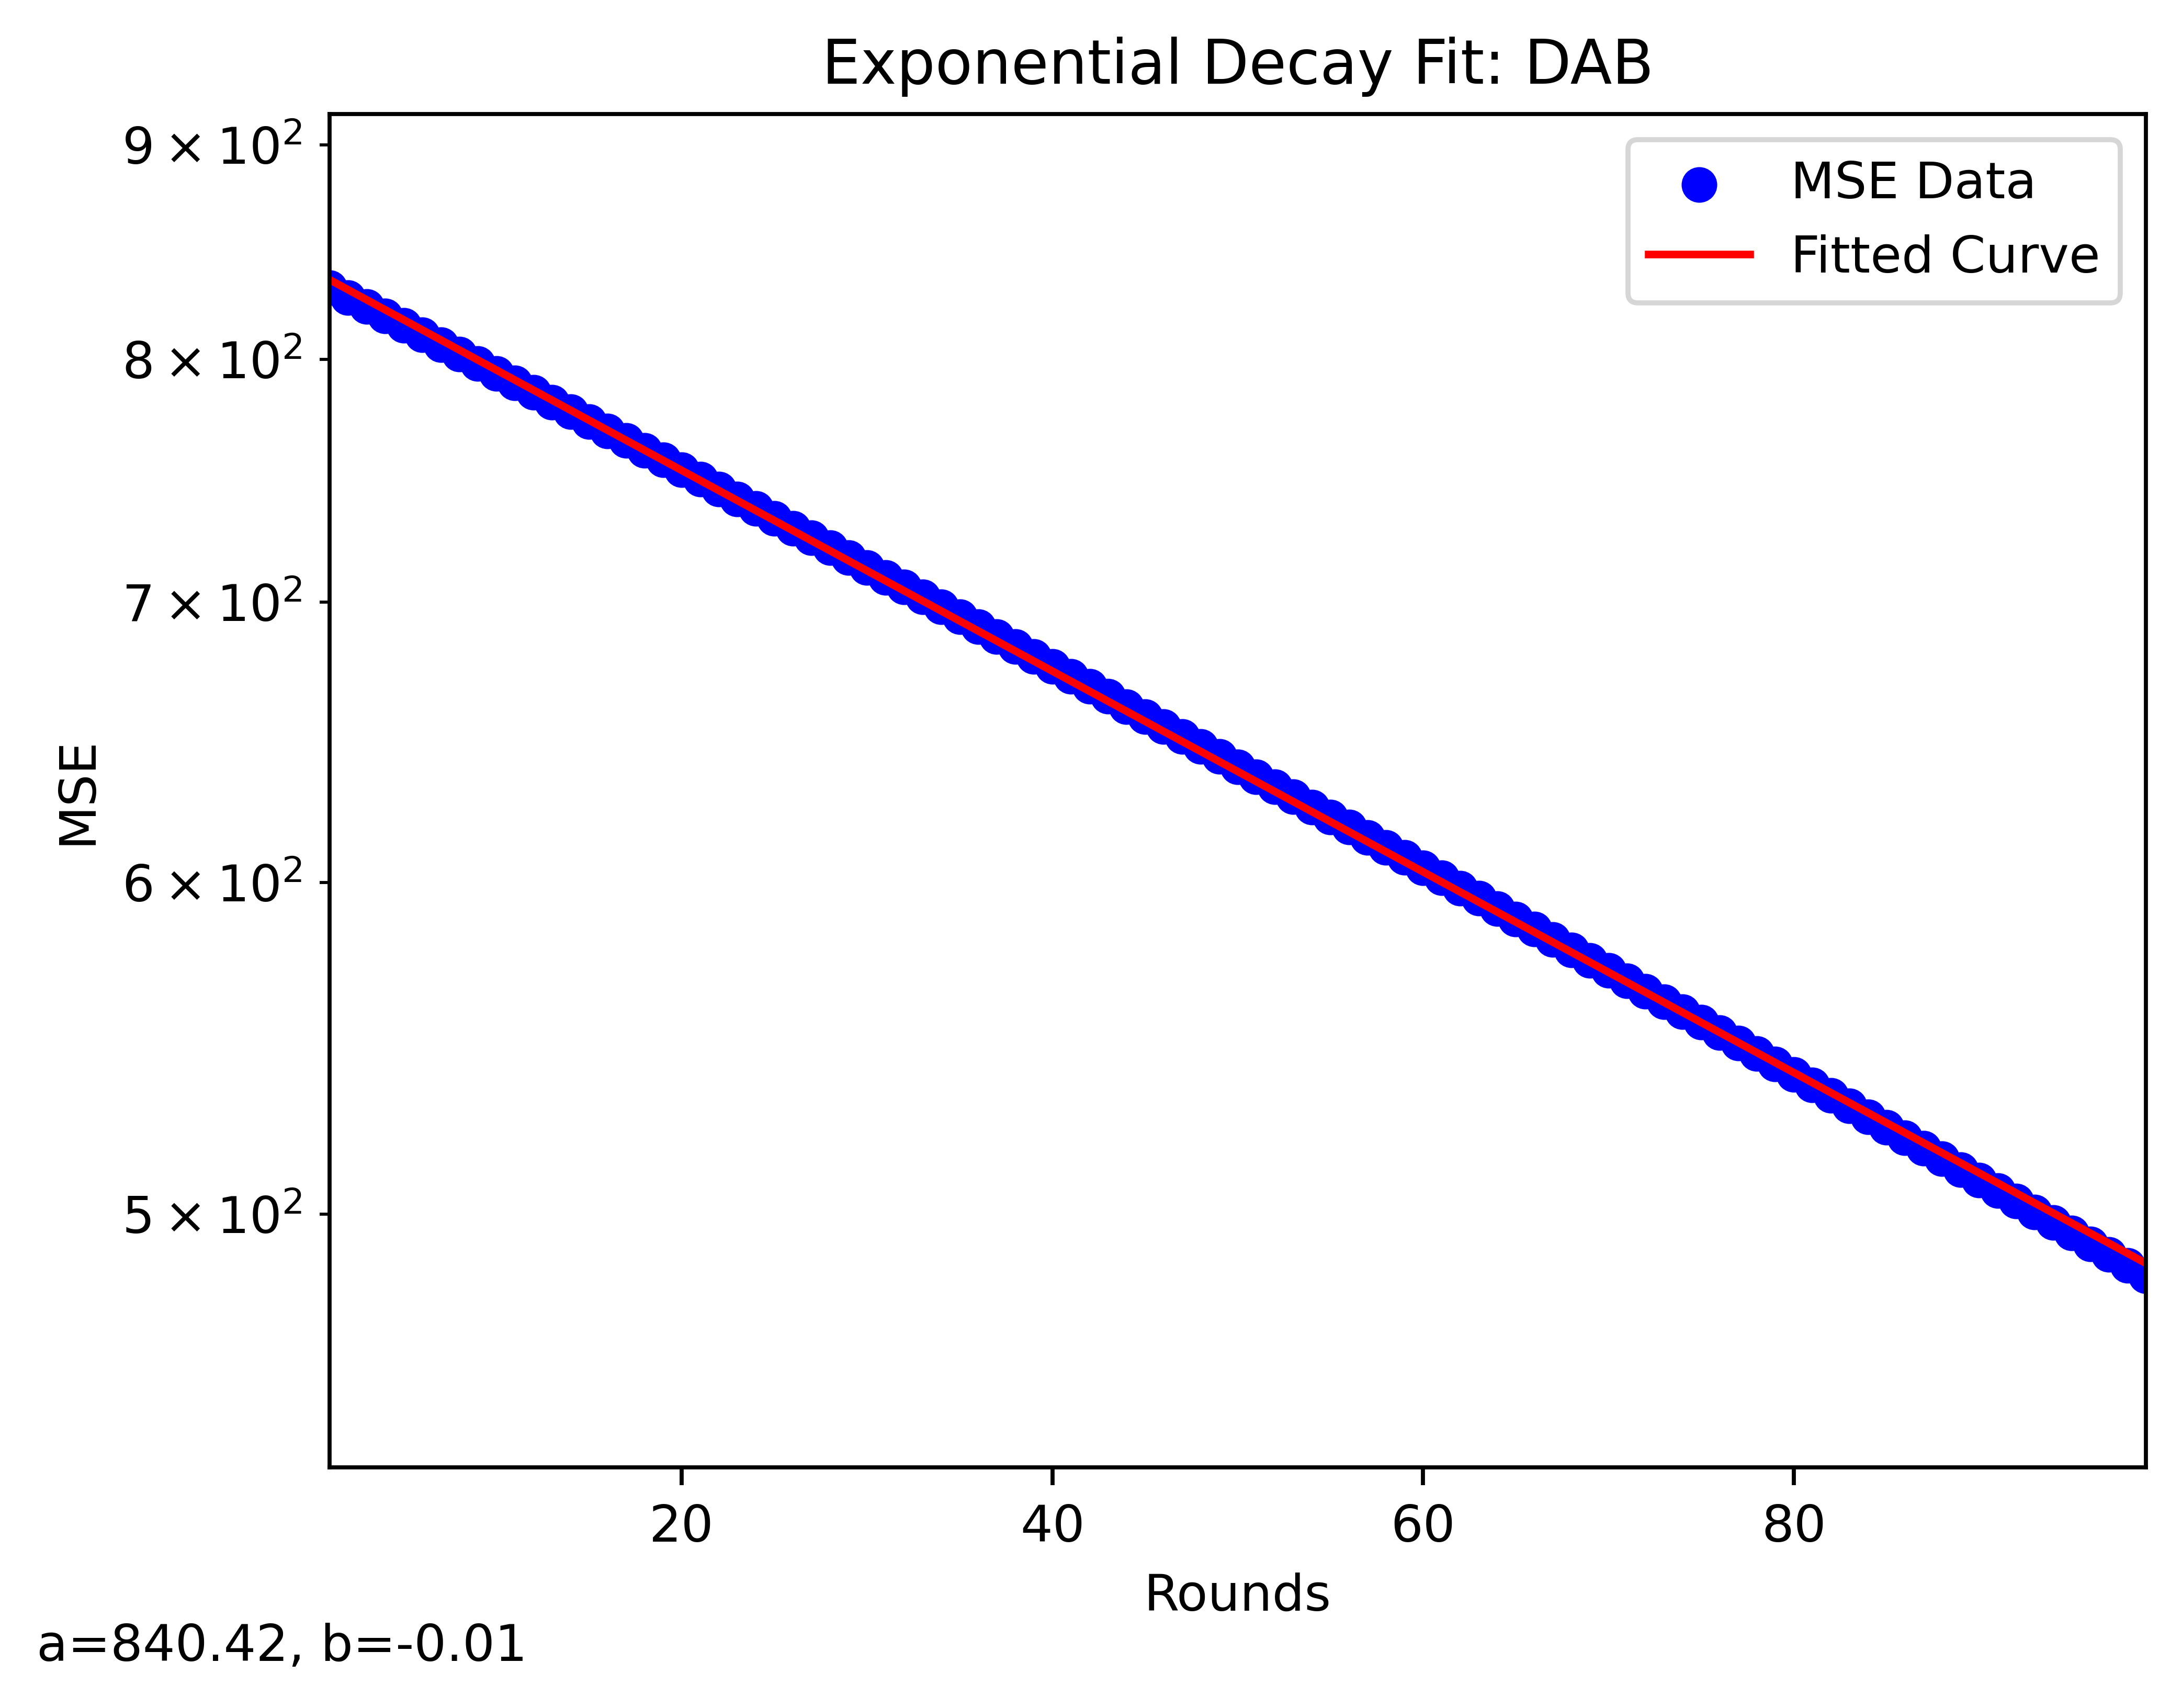
\includegraphics[width=\linewidth]{figures/Simulation_outcomes/StarGraph/DAB/DAB_modelfitting_rounds_99_model_1.png}
%     \caption{Exponential Decay Fit: DAB}
%     \label{fig:dabStarModelFit}
% \end{figure}


\textbf{Push-Pull Sum Algorithm and Adaptive Threshold Push-Pull Sum Algorithm}: Both push-pull-based protocols exhibit steep MSE reductions early on, as seen in the sharp downward trends in the log-log plot. The PPS algorithm outperforms the ATPPS algorithm, as it reduces MSE faster and reaches lower MSE values sooner (as of round 45) before the graph plateaus. Figures \ref{fig:ppsStarModelFit} and \ref{fig:atppsStarModelFit} show the fitted curves for the MSE data of the PPS and ATPPS load balancing algorithms respectively. The best-fit model for the MSE data of the PPS load balancing algorithm for the rounds 10 to 45 follows the equation $MSE=29794.60*e^{-1.39*x}$. The rounds 10 to 45 show the steepest decay and for that reason been fitted to exponential regression model. The decay rate of -1.39 indicates a very fast error reduction in the network, especially if compared to the DAB load balancing algorithms ability to reduce the error for star graph. The ATPPS load balancing algorithms MSE data fits best with the exponential model following the equation $MSE_r=9329.40*e^{-1.05*r}$ between the rounds 18 to 60. 

Overall the scenario is similiar to the complete graph, where the DAB reduces the error exponential with a very slow rate, while the push-pull based algorithms perform a very fast error reduction. This behaviour is captured in the heat map of figure \ref{fig:stargraphslopes}. While the DAB load balancing algorithm reduces the error in average per region $-3.75 \pm 0.55$, the push-pull based algorithms exhibit a error reduction of -92 for the first 10 rounds. The slopes approach zero in the middle and end regions, implying almost negligible MSE reduction in later stages. This is due to the fact that the network already is balanced to a degree where the MSE will not improve significantly further for later rounds. Both algorithms converge early and maintain a near-steady state afterward. The DAB load balancing algorithms deterministic nature and lack of adaptability lead to slower convergence and less effective load balancing, as reflected in its consistently shallow slopes.

% \begin{figure}[H]
%     \centering
%     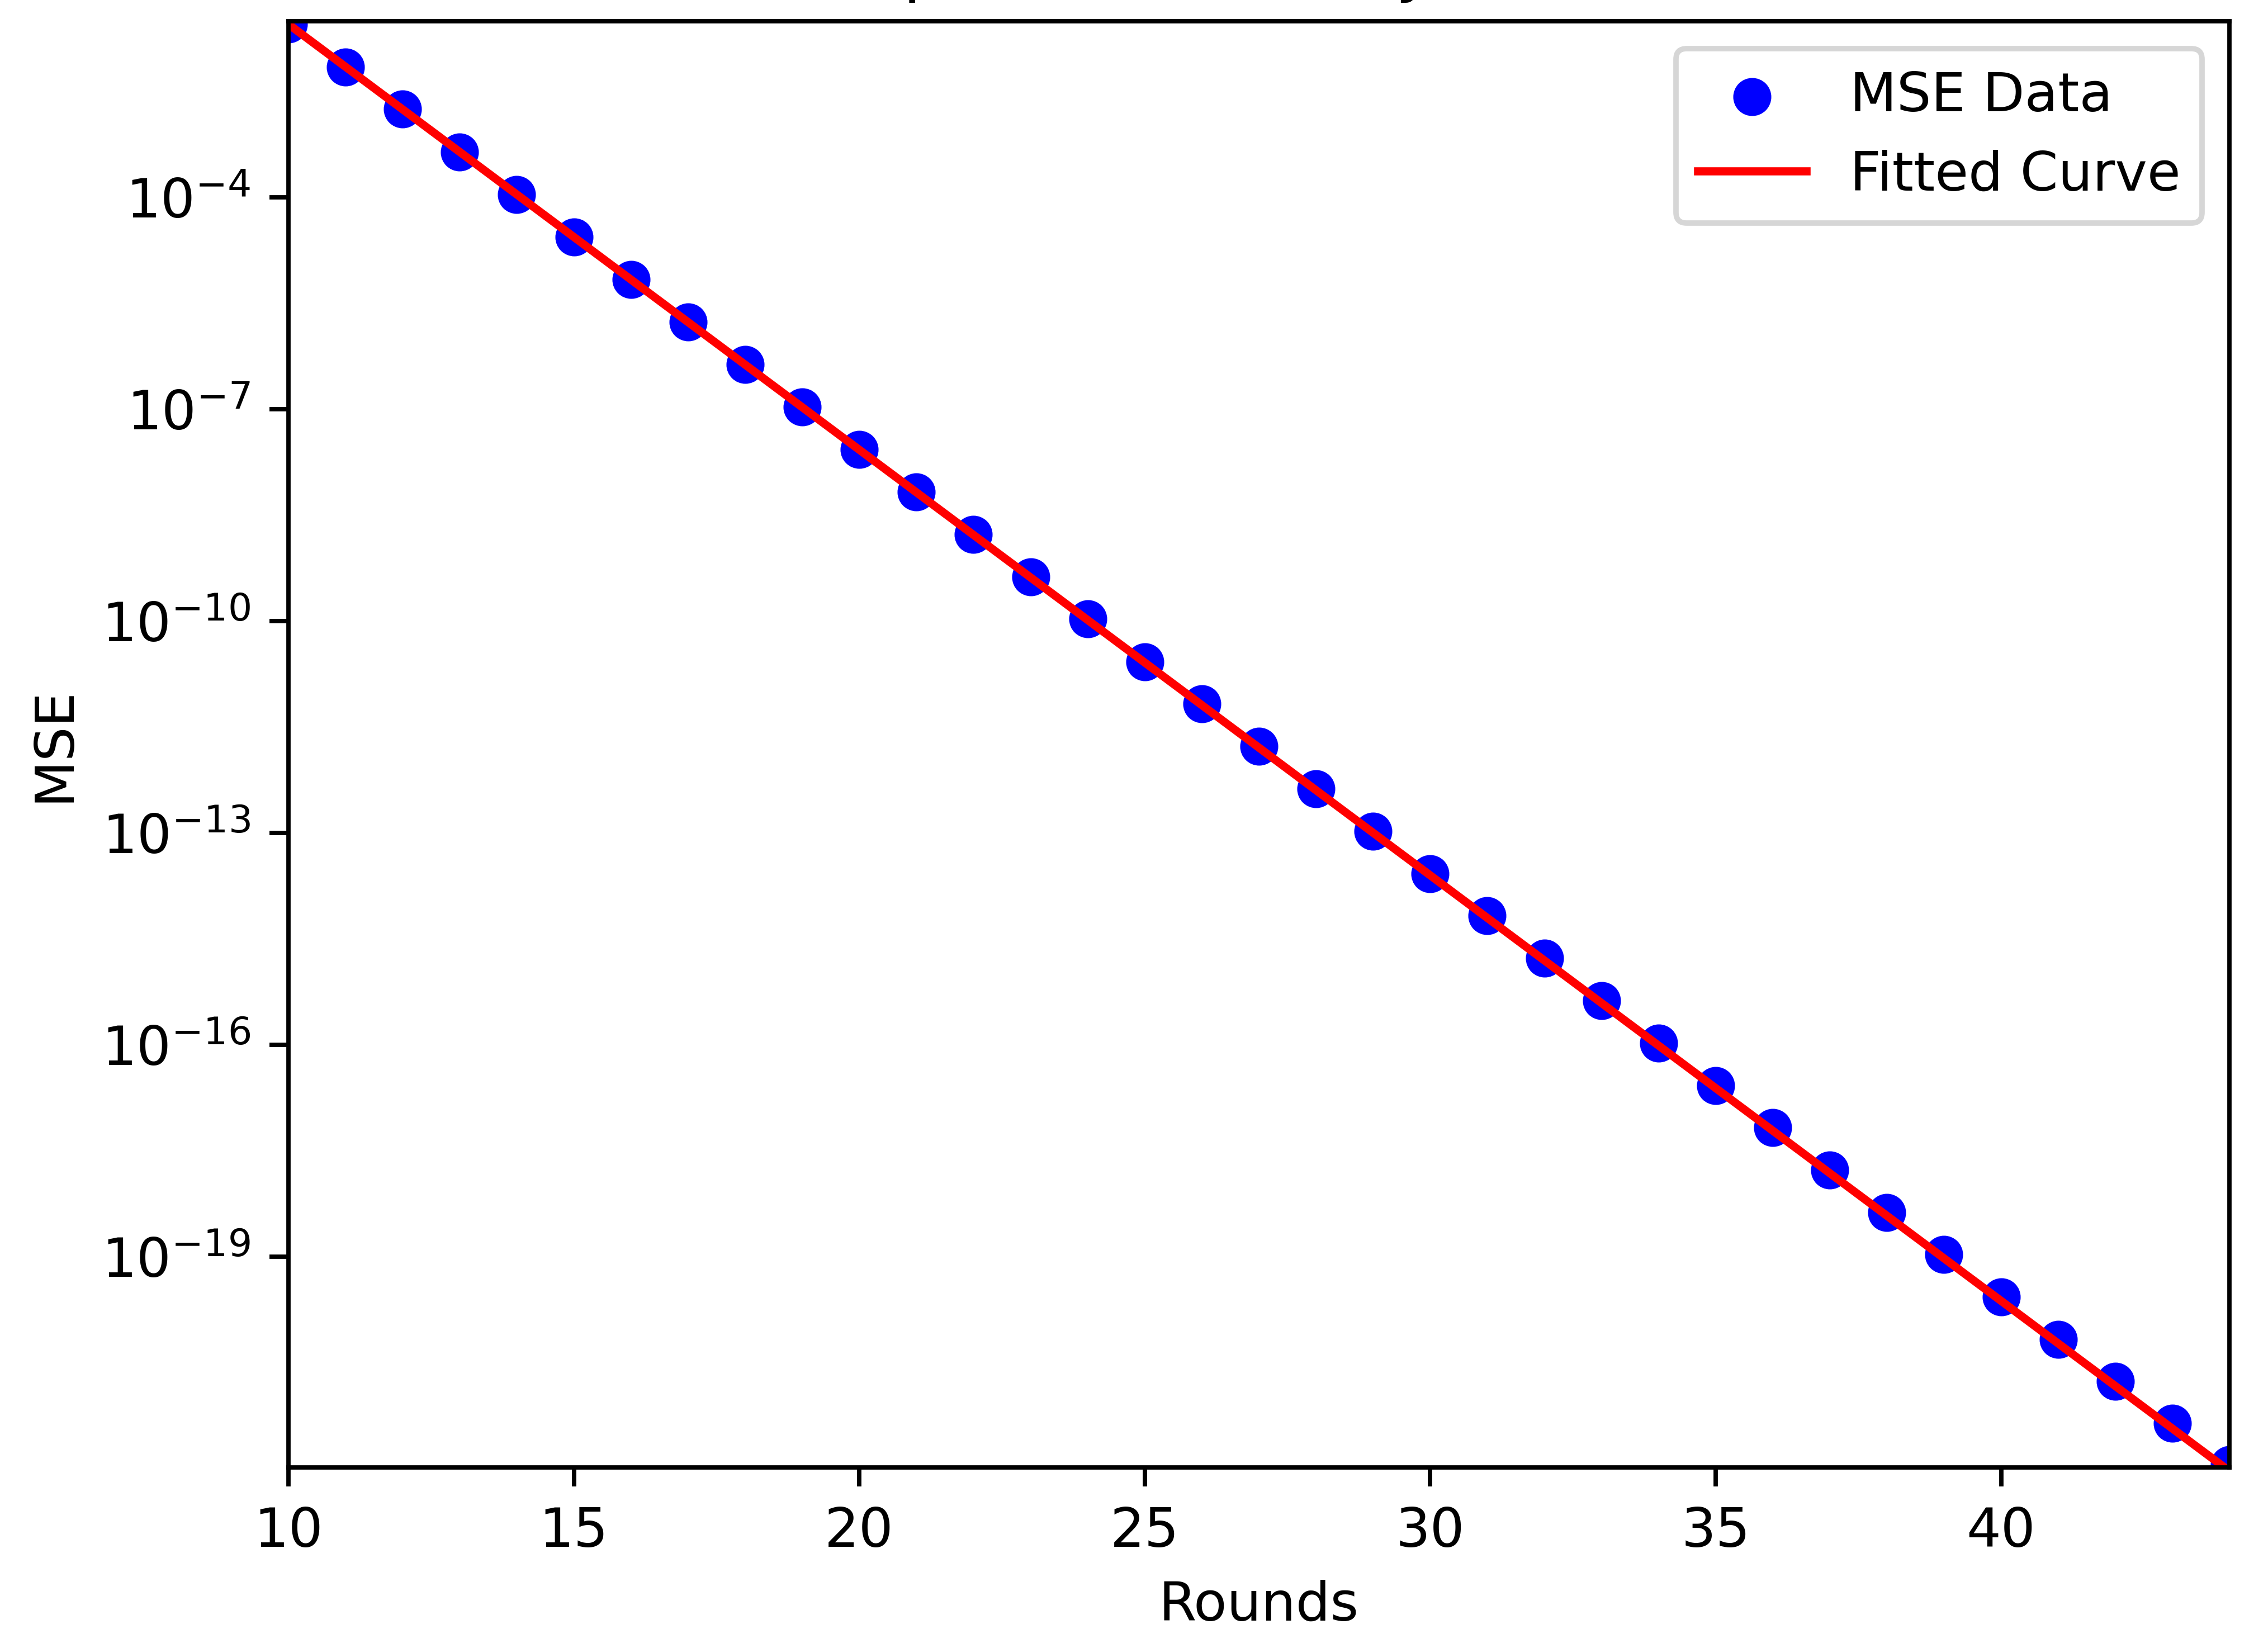
\includegraphics[width=\linewidth]{figures/Simulation_outcomes/StarGraph/PPS/PPS_modelfitting_rounds_44_model_1.png}
%     \caption{Exponential Decay Fit: PPS}
%     \label{fig:ppsStarModelFit}
% \end{figure}

% \begin{figure}[H]
%     \centering
%     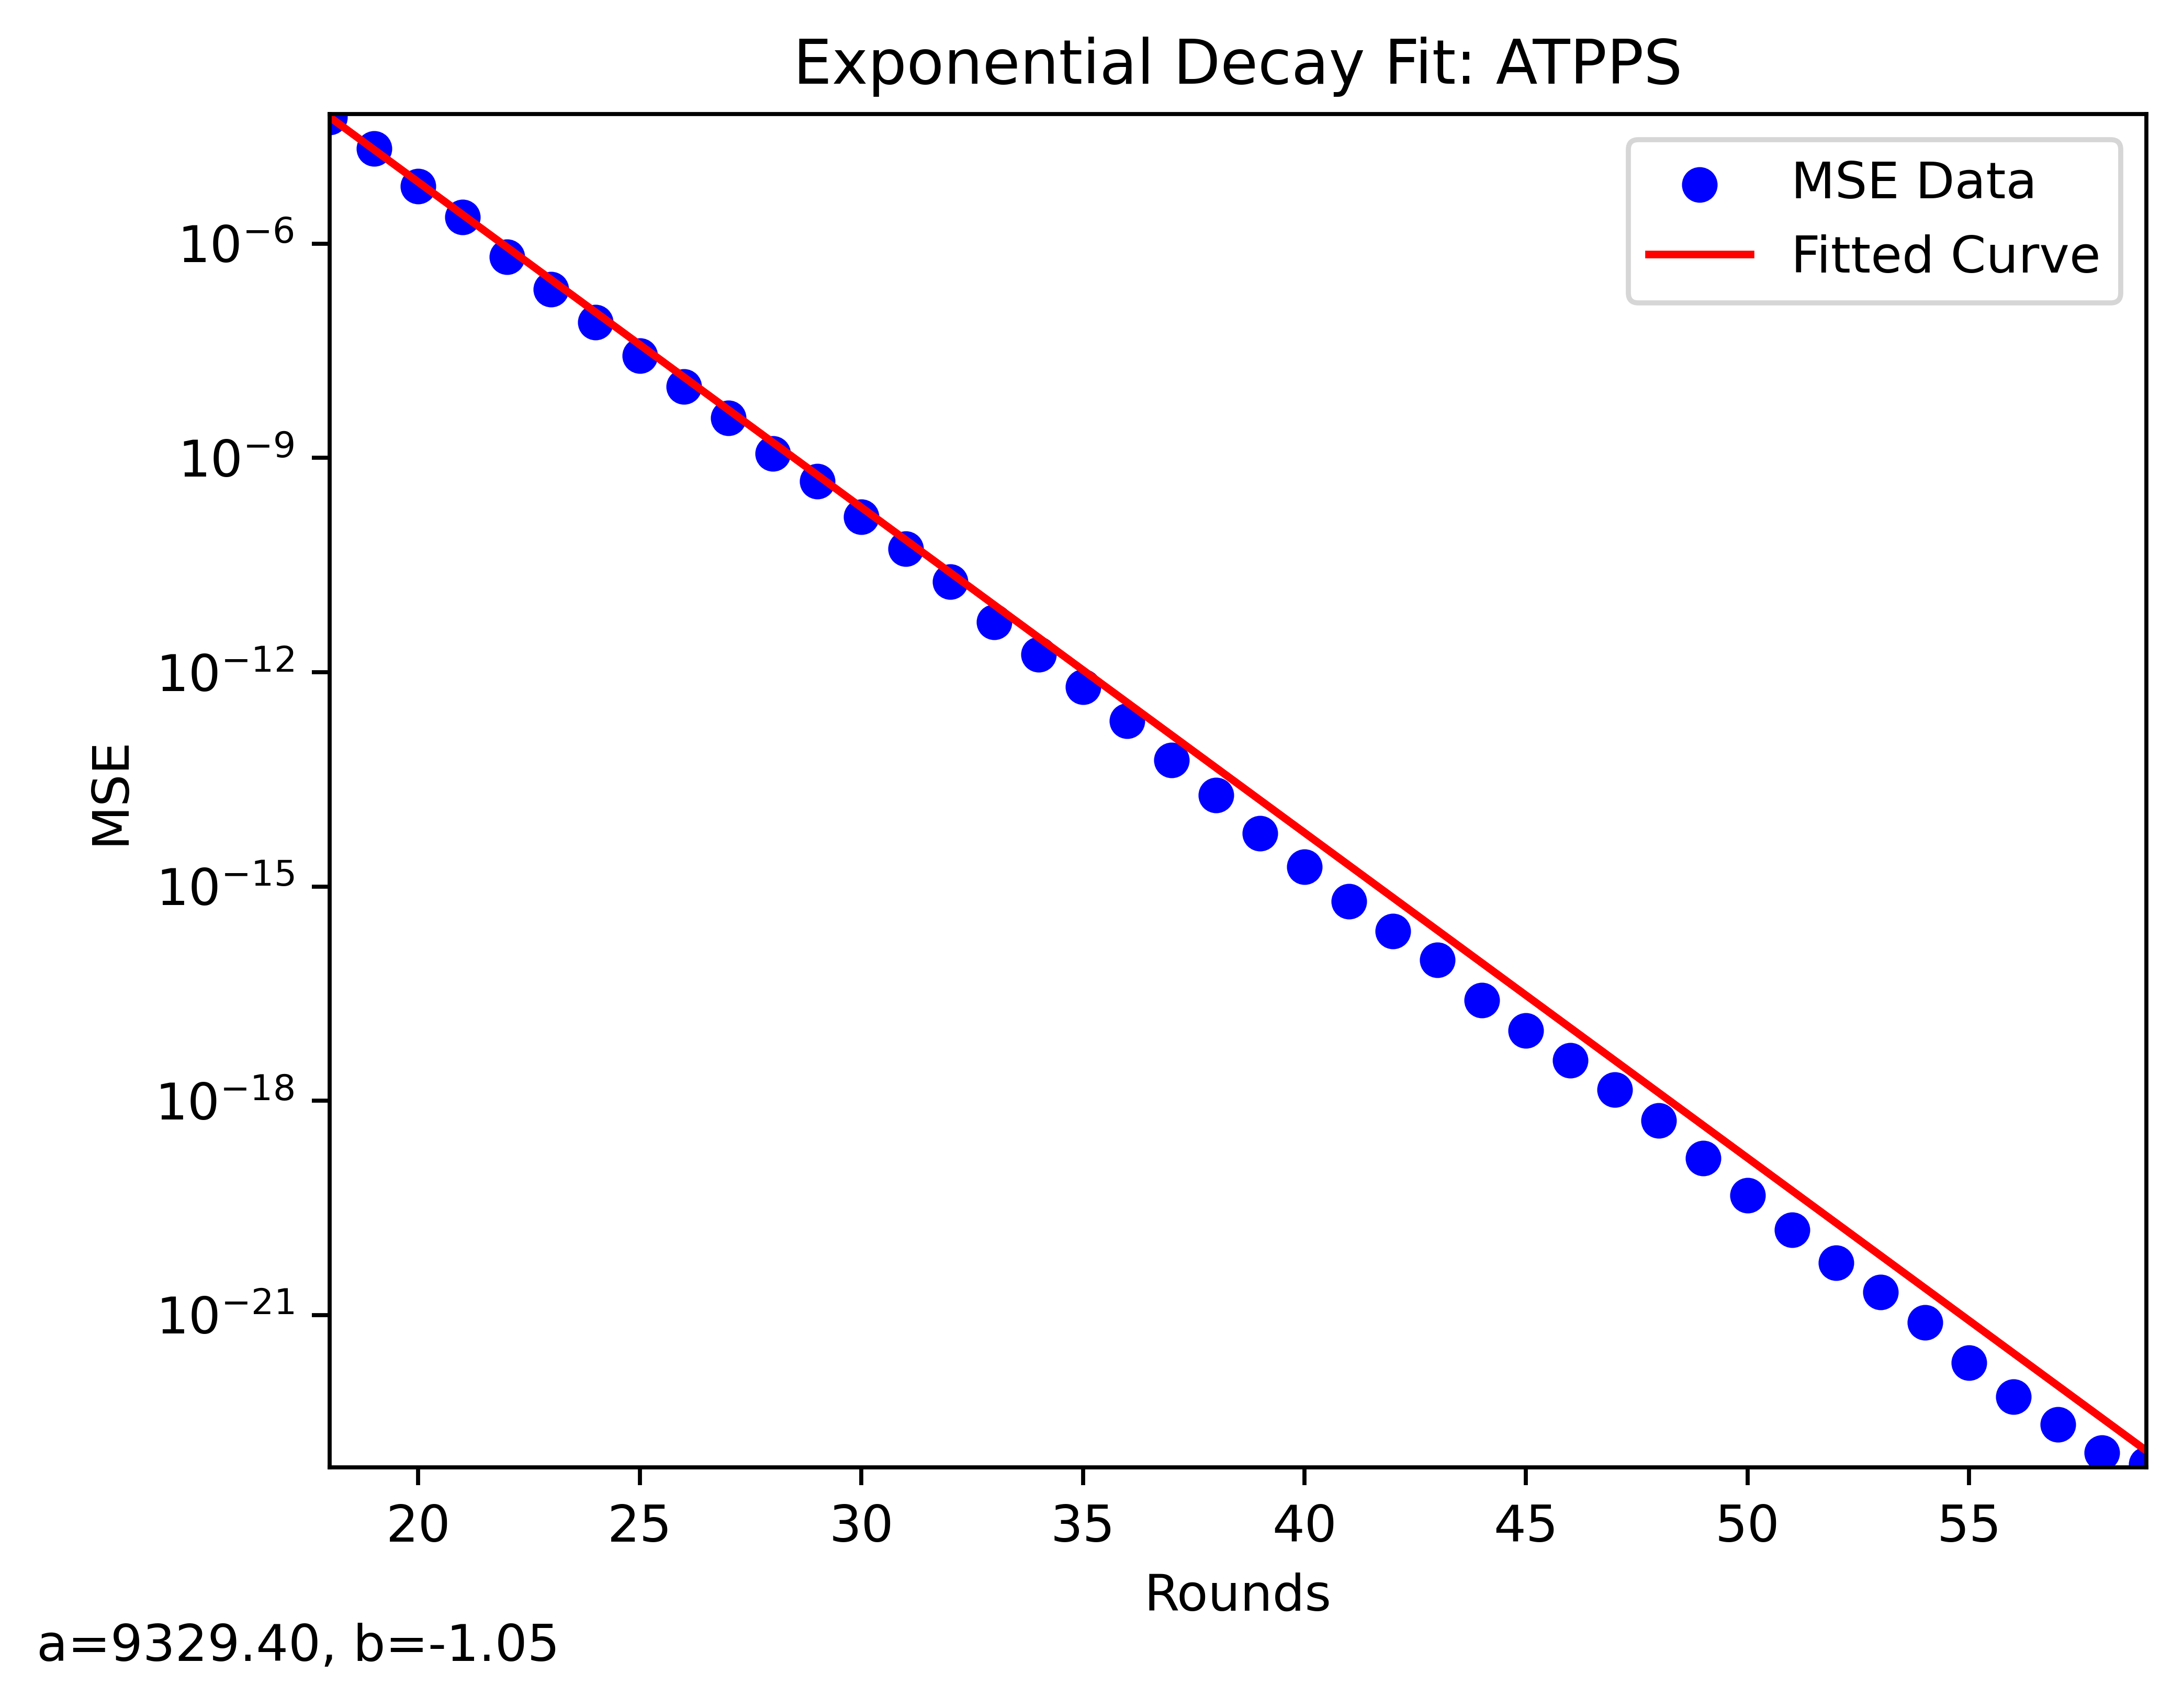
\includegraphics[width=\linewidth]{figures/Simulation_outcomes/StarGraph/ATPPS/ATPPS_modelfitting_rounds_59_model_1.png}
%     \caption{Exponential Decay Fit: ATPPS}
%     \label{fig:atppsStarModelFit}
% \end{figure}

% \begin{figure}
%     \centering
%     \scalebox{0.8}{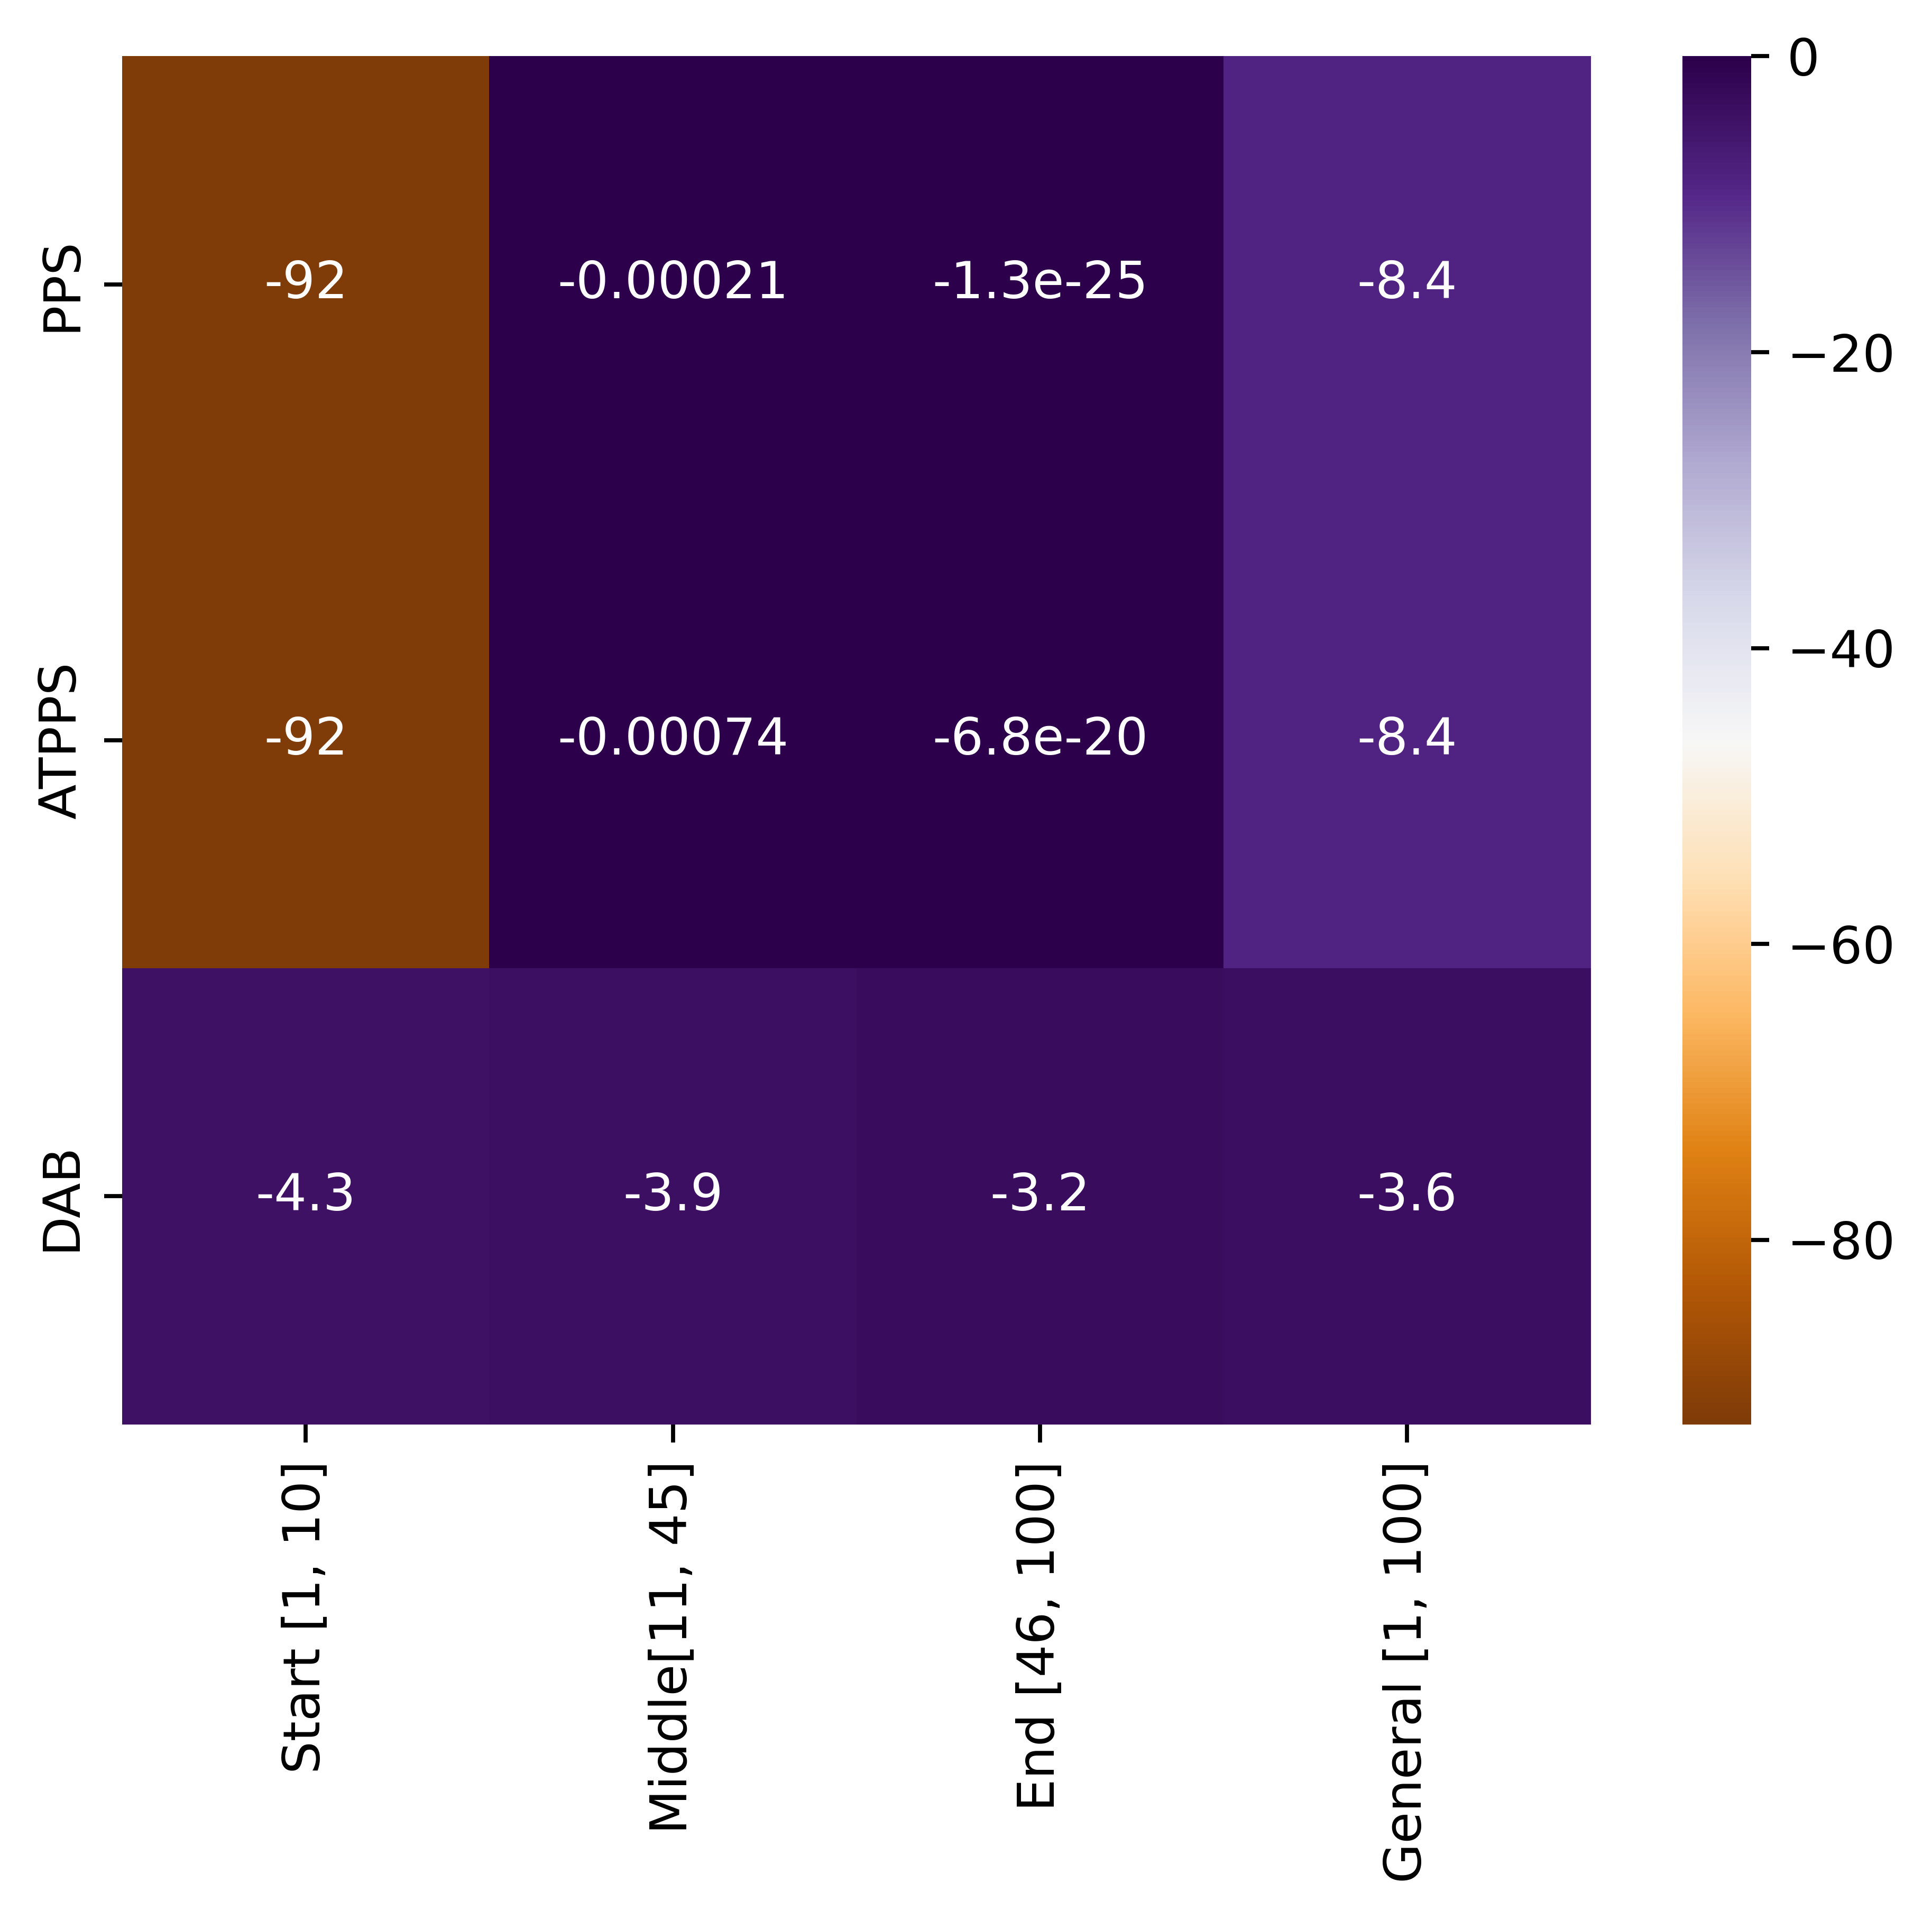
\includegraphics{figures/Simulation_outcomes/StarGraph/DAB_vs_PPS_vs_ATPPS_slopesheatmap_100rounds.png}}
%     \caption{Star Graph: heat map of slopes per region}
%     \label{fig:stargraphslopes}
% \end{figure}

\section{Ring Graph}\label{sec:ringgraph}
% \begin{figure}
%     \centering
%     \scalebox{0.5}{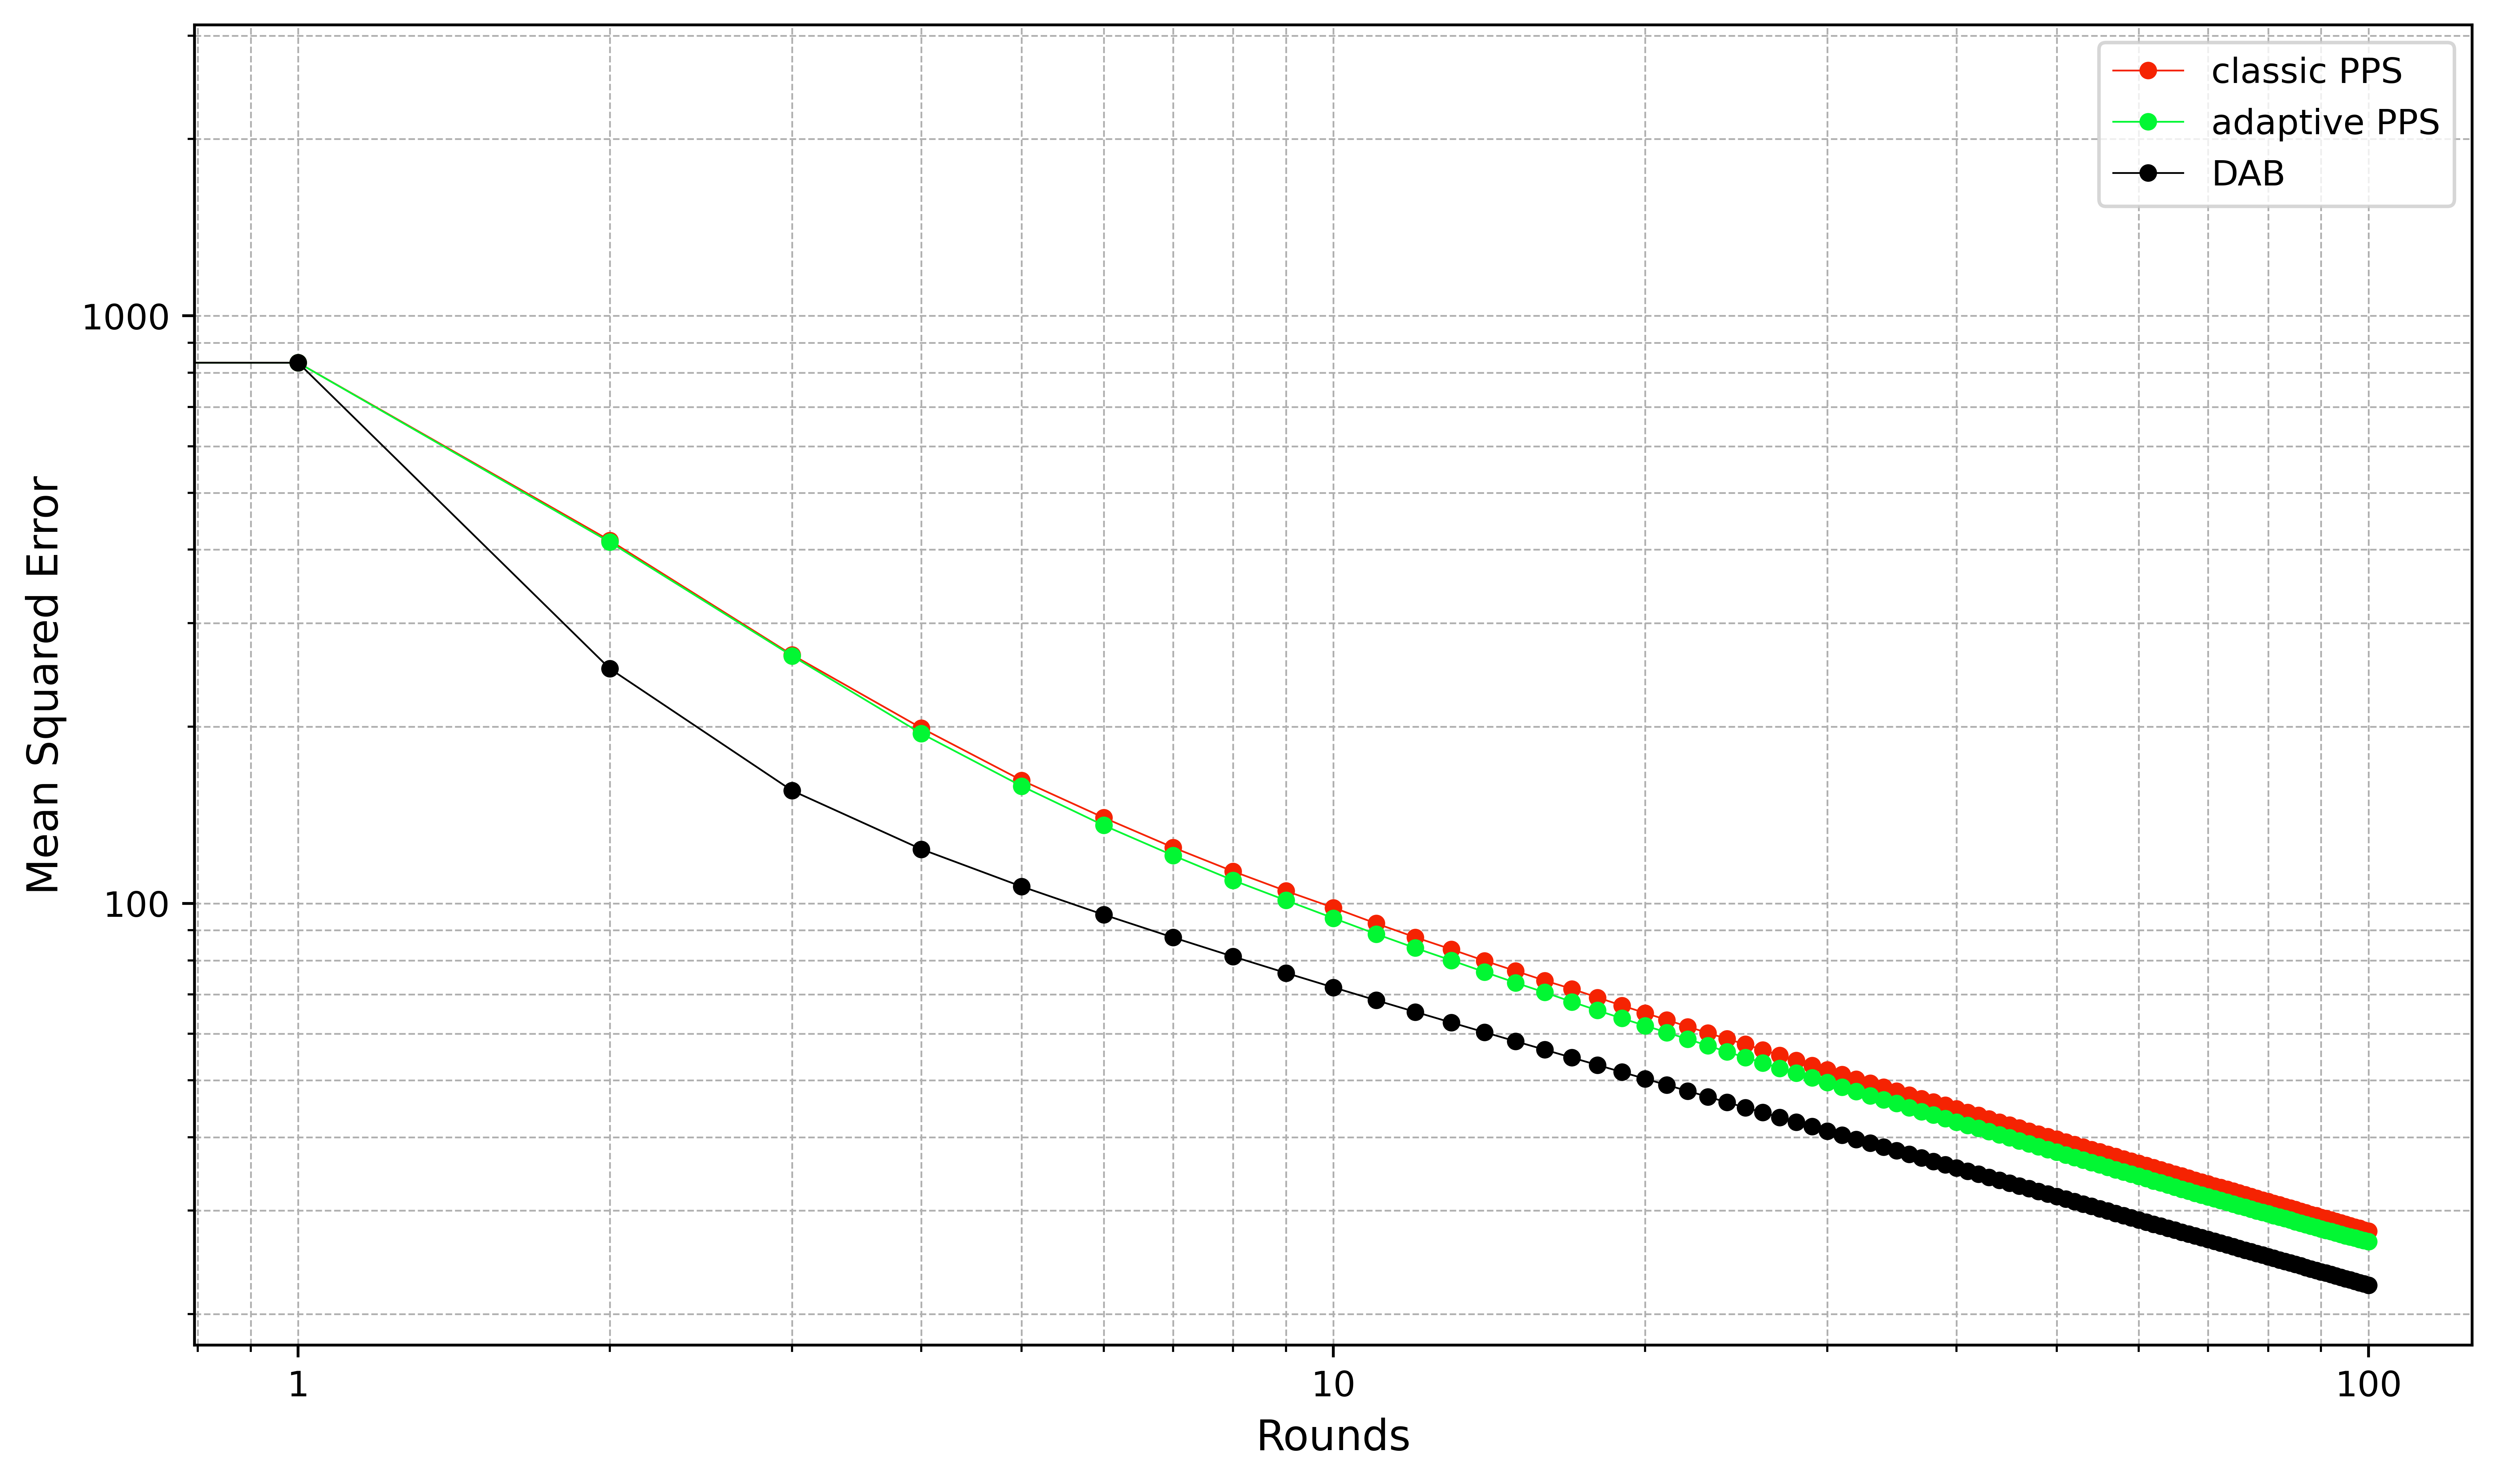
\includegraphics{figures/Simulation_outcomes/RingGraph/DAB_vs_PPS_RG_r100_n1024_averaged_loglog.png}}
%     \caption{Ring Graph: mean squared error per rounds (log-log)}
%     \label{fig:ringGraphLogLogMSEperRound}
% \end{figure}
% \begin{figure}
%     \centering
%     \scalebox{0.5}{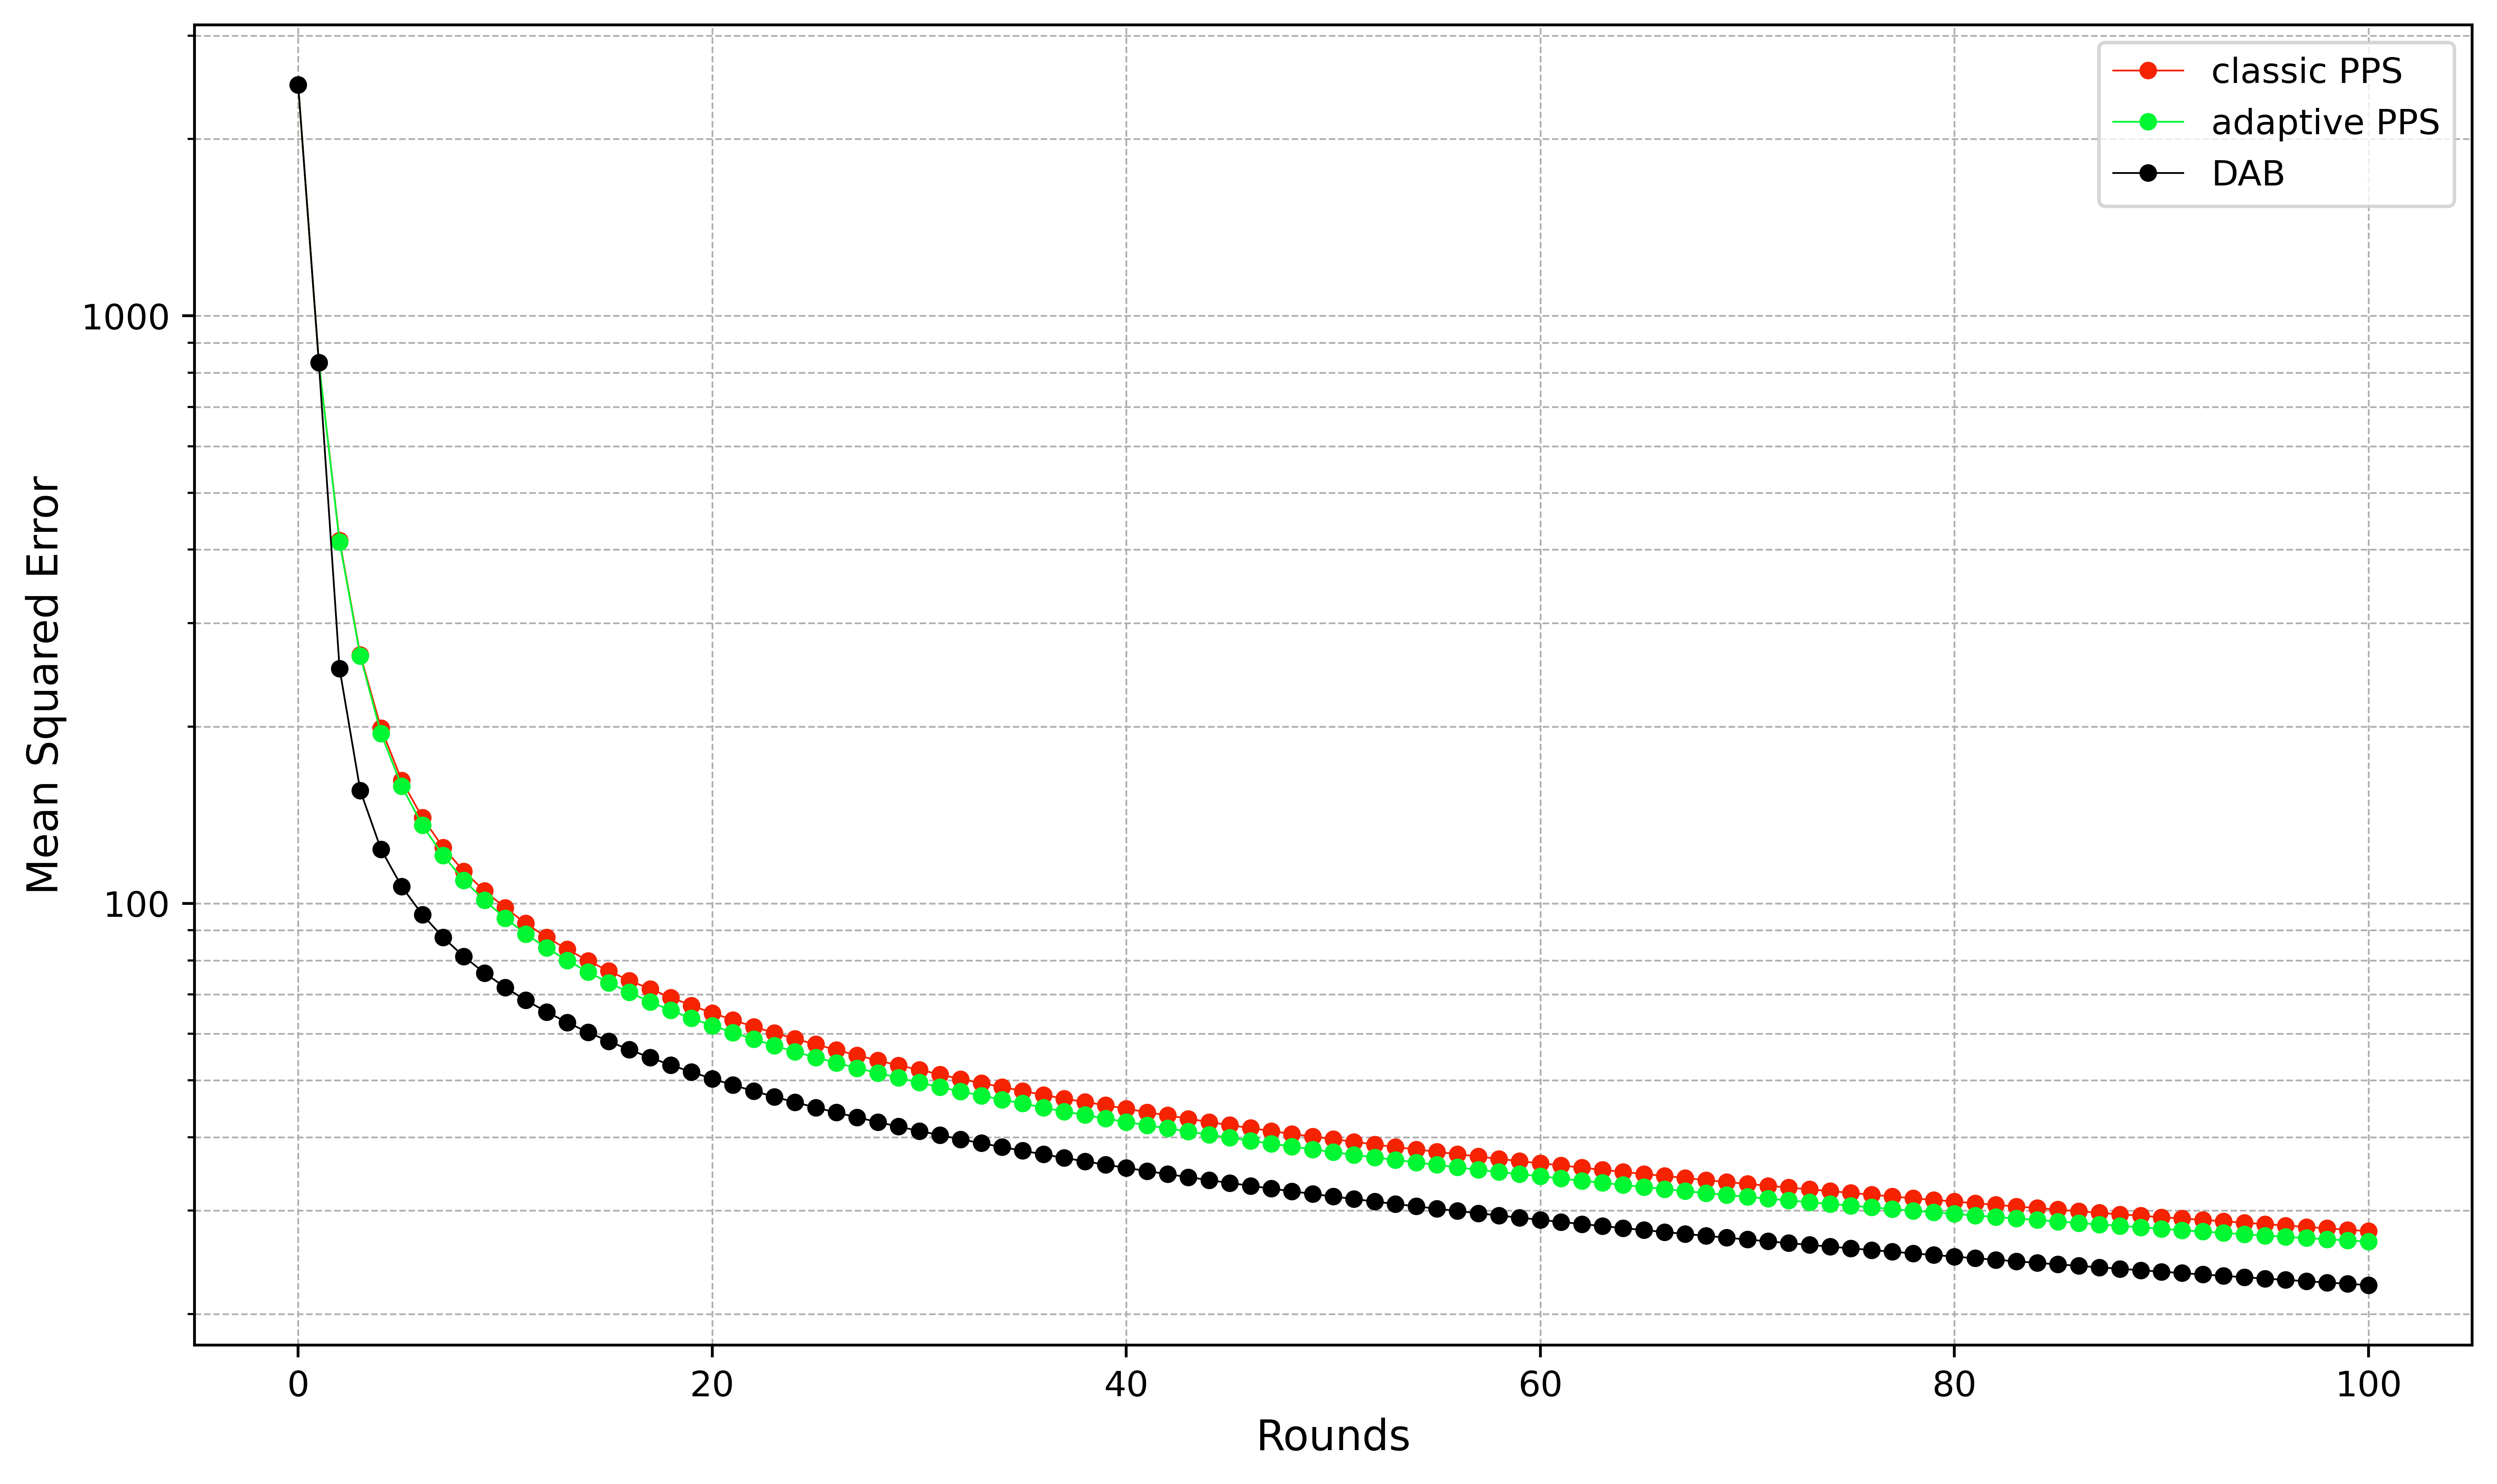
\includegraphics{figures/Simulation_outcomes/RingGraph/DAB_vs_PPS_RG_r100_n1024_averaged_log.png}}
%     \caption{Ring Graph: mean squared error per rounds (log-linear)}
%     \label{fig:ringGraphLogMSEperRound}
% \end{figure}

\section{Torus Grid Graph}\label{sec:torusgridGraph}
% \begin{figure}
%     \centering
%     \scalebox{0.5}{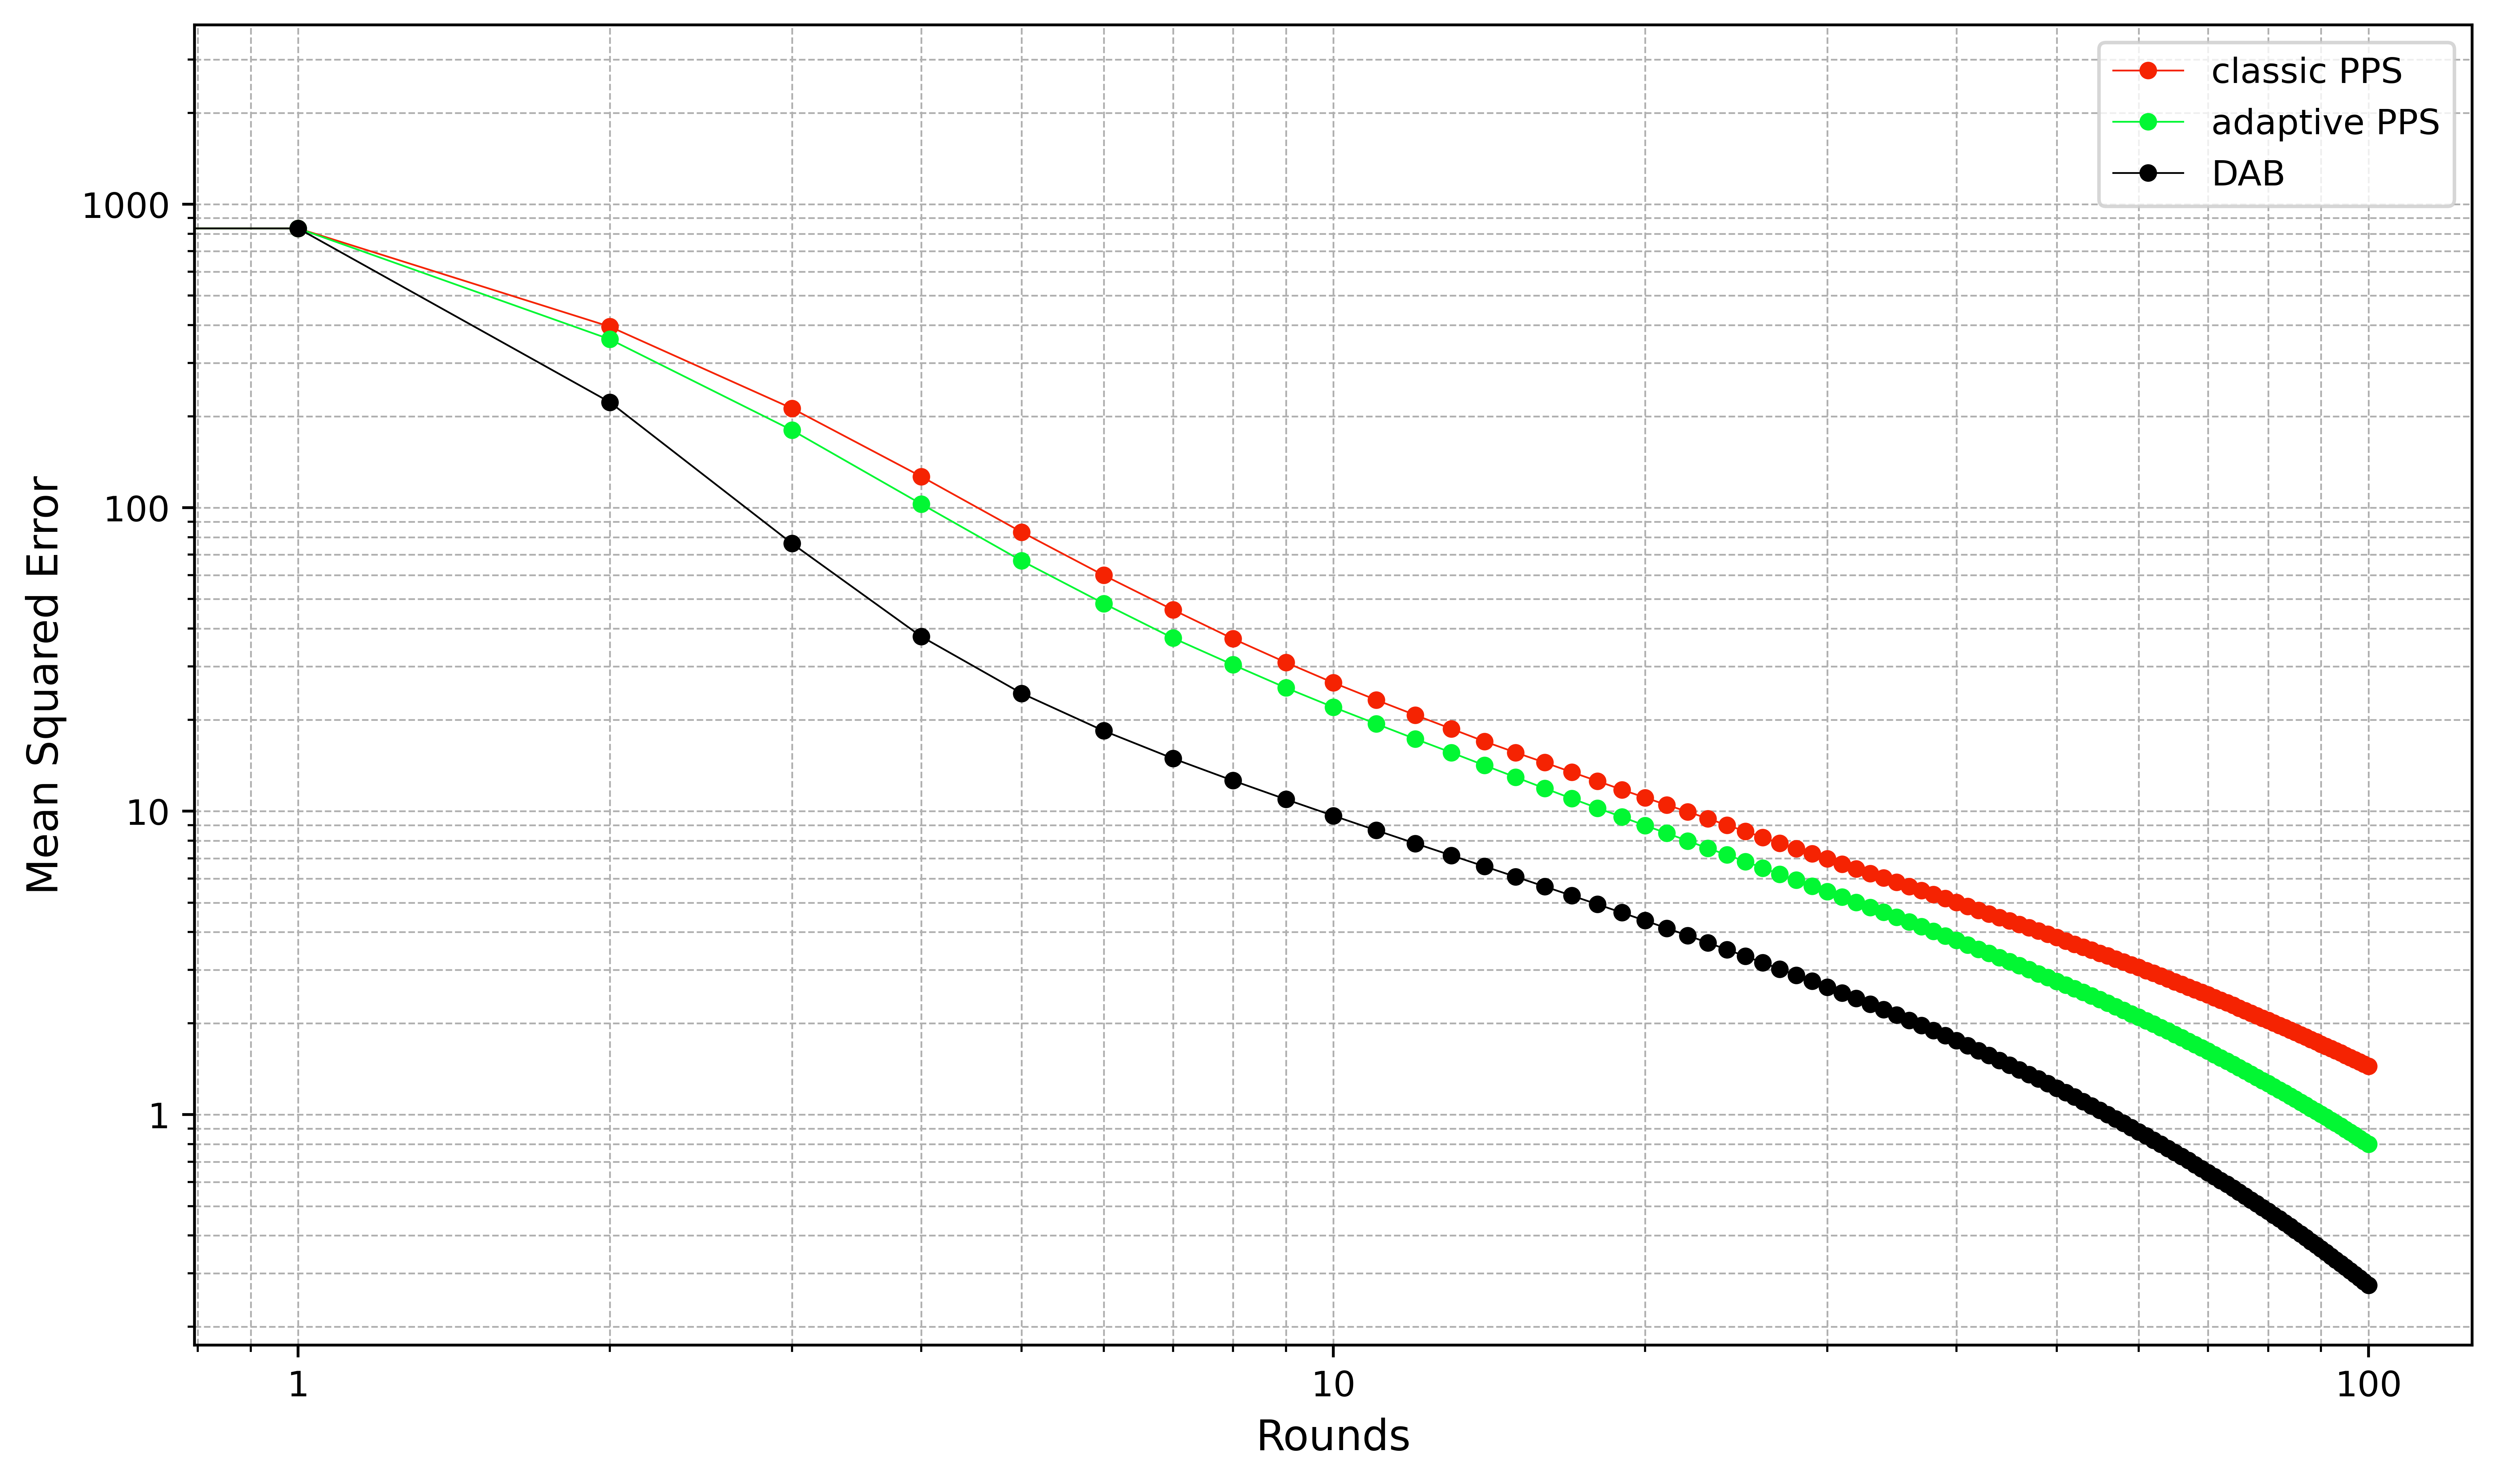
\includegraphics{figures/Simulation_outcomes/TorusGridGraph/DAB_vs_PPS_TGG_r100_n1024_averaged_loglog.png}}
%     \caption{Torus Grid Graph: mean squared error per rounds (log-log)}
%     \label{fig:torusGraphLogLogMSEperRound}
% \end{figure}

\section{Ring of Cliques}\label{sec:ringofcliques}
\section{Lollipop Graph}\label{sec:lollipopgraph}
